\lecture{Modulação por amplitude de pulso - PAM}{lec_pam}

\begin{frame}
	\begin{block}{\centering\large\bfseries Parte 3}
		\centering\large\insertpart
	\end{block}
\end{frame}


\section{PAM em banda base}

\begin{frame}
	\frametitle{PAM em banda base}

	\begin{itemize}
	    \item A escolha da modulação depende das características do meio.
	    \item Os canais podem ser classificados como: banda base (\textit{baseband}) ou banda passante (\textit{bandpass}).	\vspace{-0.3cm}  
	\end{itemize}	
	\begin{figure}[t]	
	  \begin{center}
	    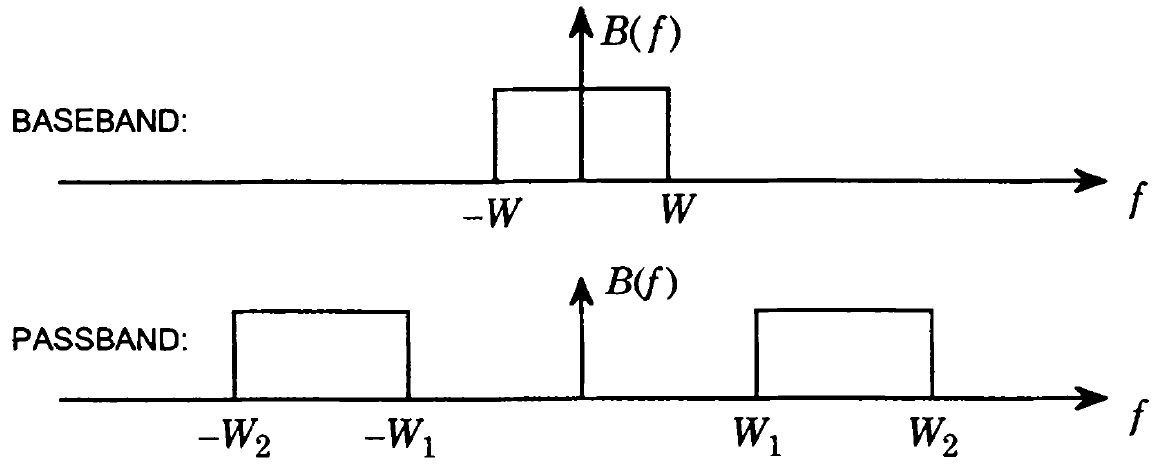
\includegraphics[width=0.5\columnwidth]{figs/pam_01}
	  \end{center}
	\end{figure}
	\vspace{-0.3cm}
	\begin{itemize}
	    \item Sinal PAM em banda base:\vspace{-0.3cm}
	\end{itemize}
	\begin{columns}
		\begin{column}{0.5\textwidth}
		    \begin{equation*}
			s(t) = \sum\limits_{m=-\infty}^{\infty} a_k g(t-kT)
		    \end{equation*}
		\end{column}
		\begin{column}{0.5\textwidth}
		    \begin{itemize}
			\item Taxa de símbolo: $1/T$
			\item Pulso de transmissão: $g(t)$
			\item Símbolos: $\{a_k\}$
		    \end{itemize}
		\end{column}
	\end{columns}	
\end{frame}

\begin{frame}
	\frametitle{PAM em banda base}

	\begin{figure}[t]	
	  \begin{center}
	    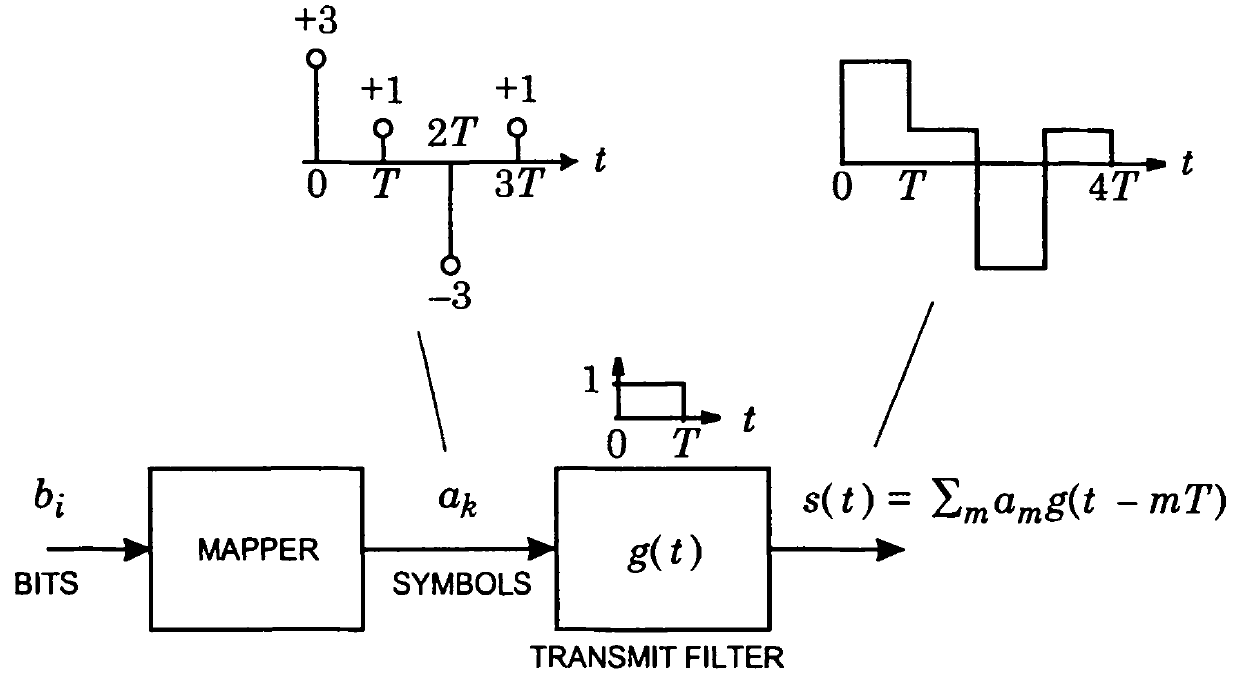
\includegraphics[width=0.5\columnwidth]{figs/pam_02}
	  \end{center}
	\end{figure}	
	\begin{itemize}
	    \item O sinal PAM pode ser interpretado como uma sequência de pulsos superpostos com a amplitude do $k$-ésimo pulso determinada pelo $k$-ésimo símbolo.
	    \item Sequência de bits de entrada é mapeada em uma sequência de símbolos $\{a_k\}$ por um \textit{mapeador}.
	    \item Os símbolos são restritos a um alfabeto finito $\mathcal{A}$, de forma que $a_k \in \mathcal{A}$ e $|\mathcal{A}| = 2^b$, para um inteiro $b$.
	\end{itemize}			
\end{frame}

\begin{frame}
	\frametitle{PAM em banda base}

	\begin{figure}[t]	
	  \begin{center}
	    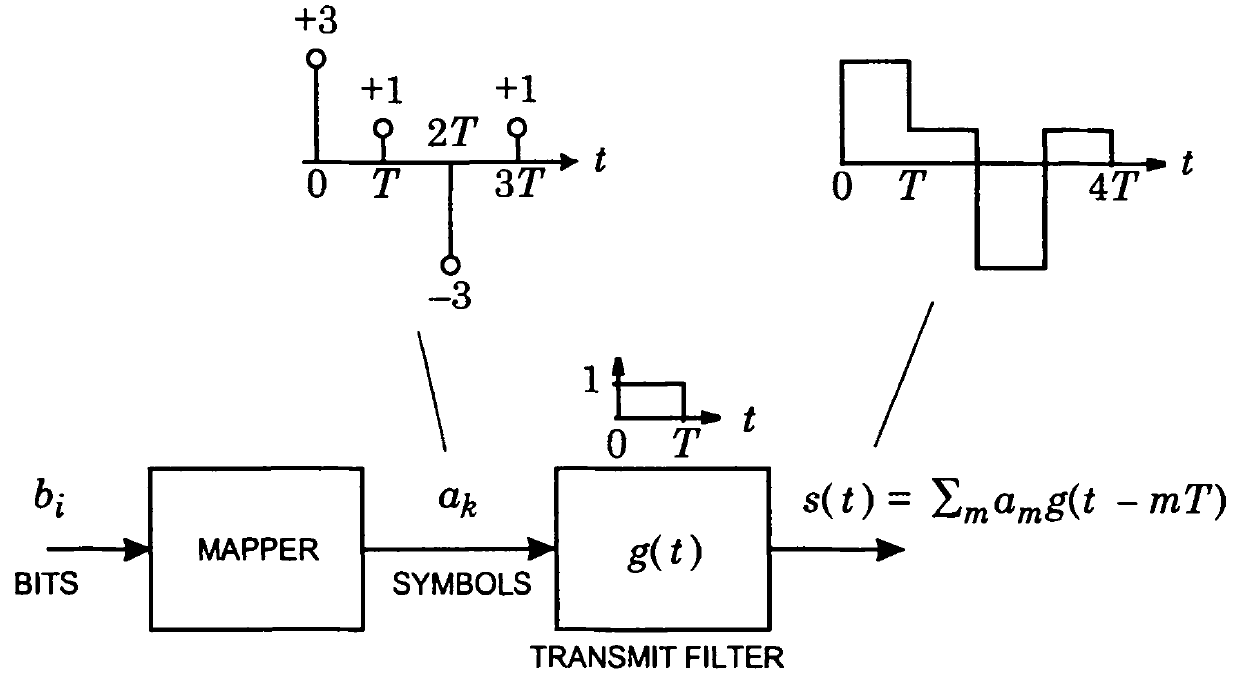
\includegraphics[width=0.5\columnwidth]{figs/pam_02}
	  \end{center}
	\end{figure}	
	\begin{itemize}
	    \item A taxa de símbolos $1/T$ também é chamada de \textit{baud rate}.
	    \item O mapeamento pode ser precedido por uma etapa de codificação de canal, na qual é adicionada redundância à sequência de bits, de forma a reduzir os erros.
	    \item Nesta disciplina vamos assumir que os símbolos que resultam do mapeamento são \textit{iid} (independentes e identicamente distribuídos).
	\end{itemize}			
\end{frame}

\begin{frame}
	\frametitle{Formatação de pulso}

	\begin{itemize}
	    \item Vamos considerar nessa seção o caso sem ruído, tendo como objetivo determinar a relação entre a largura de banda e a taxa de símbolos.
	    \item Considere a amostragem de $s(t)$ em múltiplos inteiros do tempo de símbolo:
	    \begin{align*}
		s(kT) &= \sum\limits_{m=-\infty}^{\infty} a_m g(kT-mT) = a_k * g(kT) \\
		&= \underbrace{a_k g(0)}_{\text{\textcolor{blue}{Termo desejado}}} + \underbrace{\sum\limits_{m\neq k} a_m g(kT-mT)}_{\text{\textcolor{red}{Interferência Inter-simbólica (ISI)}}}
	    \end{align*}
	    \item Condição para que a ISI seja anulada:
	    \begin{equation*}
		    g(kT) = \delta_k
	    \end{equation*}
	\end{itemize}			
\end{frame}

\begin{frame}
	\frametitle{Formatação de pulso}

	\begin{itemize}
	    \item Aplicando a transformada de Fourier obtemos:
	    \begin{equation*}
		    g(kT) = \delta_k \quad \xrightarrow{\mathcal{F}} \quad \frac{1}{T}\sum\limits_{m=-\infty}^{\infty} G\left(f-\frac{m}{T} \right) = 1
	    \end{equation*}
	    \item Obtemos portanto o \textcolor{blue}{\textit{critério de Nyquist}}.
	    \item Um pulso que satisfaz esse critério é chamado de \textit{pulso de Nyquist}.
	    \item Este critério implica que existe uma banda mínima a ser respeitada para se transmitir a uma certa taxa sem ISI.
	\end{itemize}			
	\begin{figure}[t]	
	  \begin{center}
	    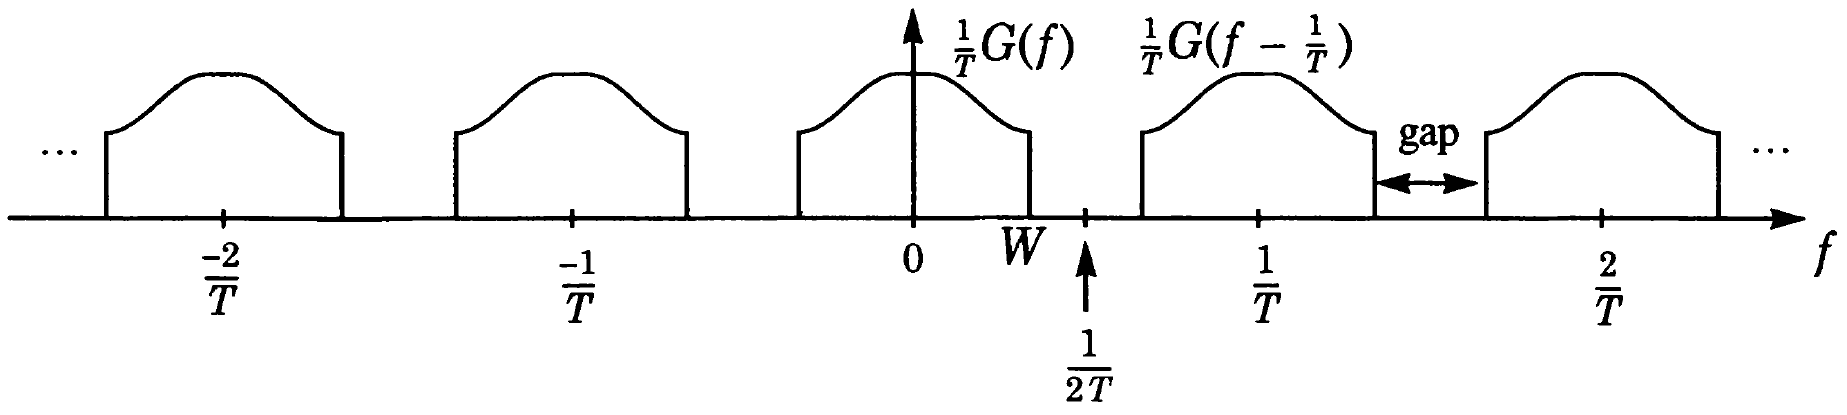
\includegraphics[width=\columnwidth]{figs/pam_03}
	  \end{center}
	\end{figure}
\end{frame}

\begin{frame}
	\frametitle{Formatação de pulso}

	\begin{itemize}
	    \item Largura de banda mínima para evitar ISI: $W \geq 1/(2T)$
	    \item Máxima taxa de símbolos correspondente: $1/T \leq 2W$
	    \item Mas não é qualquer pulso que satisfaz o critério de Nyquist: o espectro resultante deve ser uma constante.
	    \item Exemplo de pulso que satisfaz o critério:
	\end{itemize}			
	\begin{figure}[t]	
	  \begin{center}
	    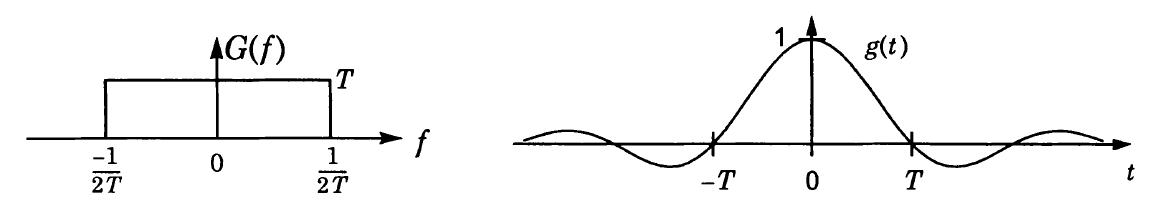
\includegraphics[width=\columnwidth]{figs/pam_04}
	  \end{center}
	\end{figure}
	\small
	$G(f) = \begin{cases}
		    T , \quad -1/(2T) \leq f \leq 1/(2T) \\
		    0, \quad \text{c.c.}
		\end{cases}  \xrightarrow{\mathcal{F}^{-1}} \quad g(t) = \frac{\sin(\pi t/T)}{\pi t/T}$

\end{frame}


\begin{frame}
	\frametitle{Formatação de pulso}

	\begin{itemize}
	    \item Ilustração de uso do pulso de Nyquist.
	    \item Considere símbolos sucessivos com valores $a_0=1$ e $a_1=2$.
	    \item Contribuição dos símbolos ao sinal:
	\end{itemize}			
	\begin{figure}[t]	
	  \begin{center}
	    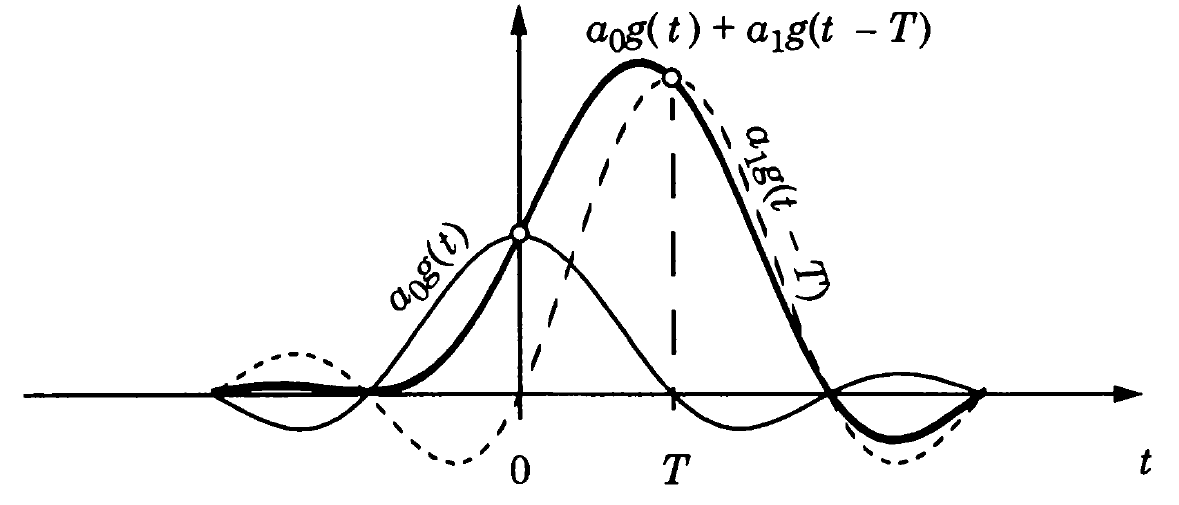
\includegraphics[width=0.7\columnwidth]{figs/pam_05}
	  \end{center}
	\end{figure}
\end{frame}


\begin{frame}
	\frametitle{Formatação de pulso}

	\begin{itemize}
	    \item O pulso ideal retangular (na frequência) possui a propriedade desejável de mínima banda, mas apresenta problemas de realização prática.
	    \item Um pulso prático deve apresentar um fator de excesso de banda $\alpha$, de forma que:
	    \begin{equation*}
		W = \frac{1+\alpha}{2T}
	    \end{equation*}
	    \item Pulso ideal ocorre para $\alpha=0$;
	    \item Valores práticos de excesso de banda: 10\% a 100\%.
	    \item Custo-benefício entre aumento de banda e simplicidade de implementação.
	    \item $\alpha$ também é chamado de fator de \textit{roll-off}.
	    \item Existem múltiplas soluções de pulsos que satisfazem o critério de Nyquist para $\alpha >0$.
	\end{itemize}			
\end{frame}

\begin{frame}
	\frametitle{Formatação de pulso}

	\begin{itemize}
	    \item Pulso cosseno levantado
	\end{itemize}
	\begin{small}
	\begin{align*}
	    g(t) &= \left( \frac{\sin(\pi t/T)}{\pi t/T} \right) \left( \frac{\cos(\alpha \pi t/T)}{1-(2\alpha t/T)^2} \right) \\
	    G(f) &= \begin{cases}
			T, & |f| \leq \frac{1-\alpha}{2T} \\
			T\cos^2\left[ \frac{\pi T}{2\alpha} \left(|f| - \frac{1-\alpha}{2T} \right) \right], & \frac{1-\alpha}{2T} < |f| \leq \frac{1+\alpha}{2T} \\
			0, & \frac{1+\alpha}{2T} < |f|
	            \end{cases}
	\end{align*}
	\end{small}
	\begin{figure}[t]	
	  \begin{center}
	    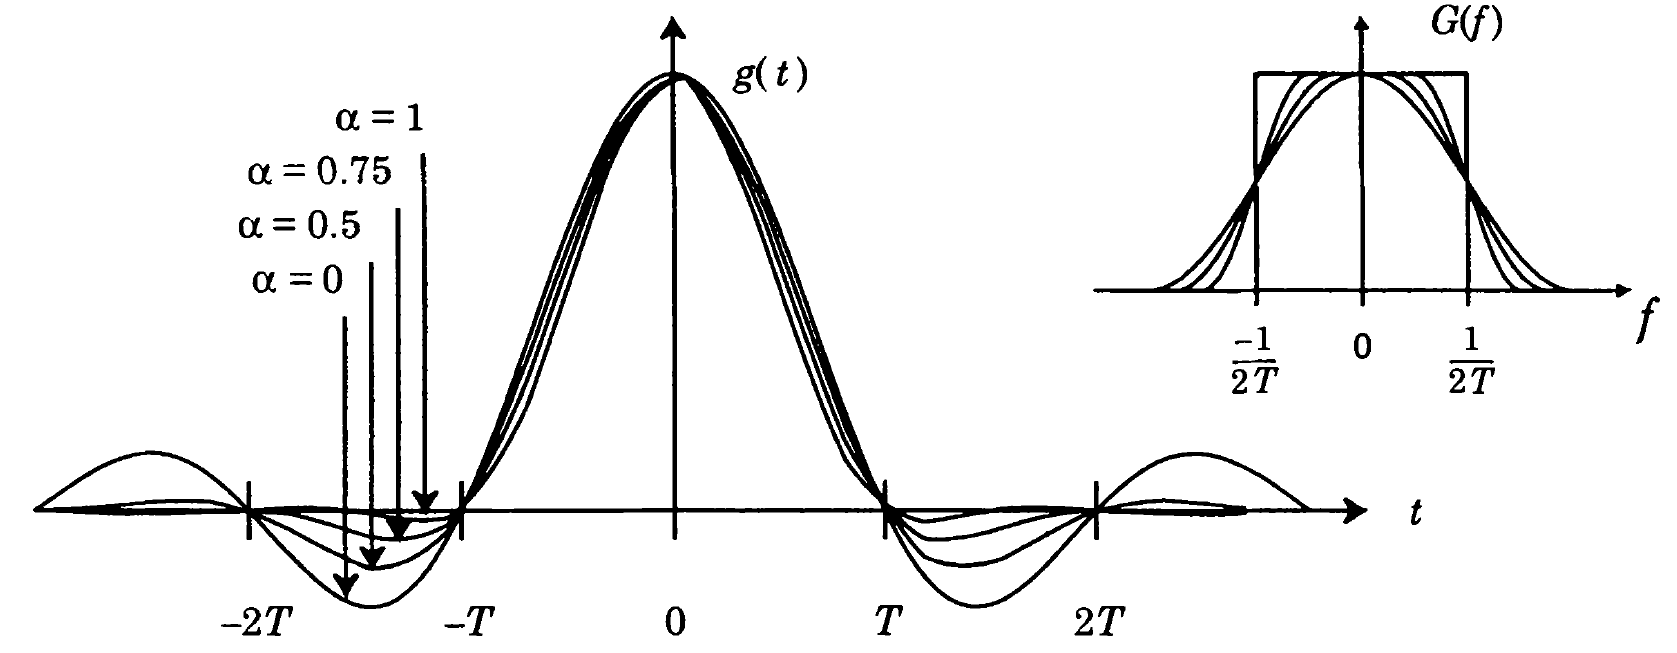
\includegraphics[width=0.8\columnwidth]{figs/pam_06}
	  \end{center}
	\end{figure}
\end{frame}

\begin{frame}
	\frametitle{Formatação de pulso}

	\begin{itemize}
	    \item Existe um número infinito de pulsos que satisfazem o critério de Nyquist.
	    \item Seguem alguns exemplos adicionais:
	\end{itemize}	
	\begin{figure}[t]	
	  \begin{center}
	    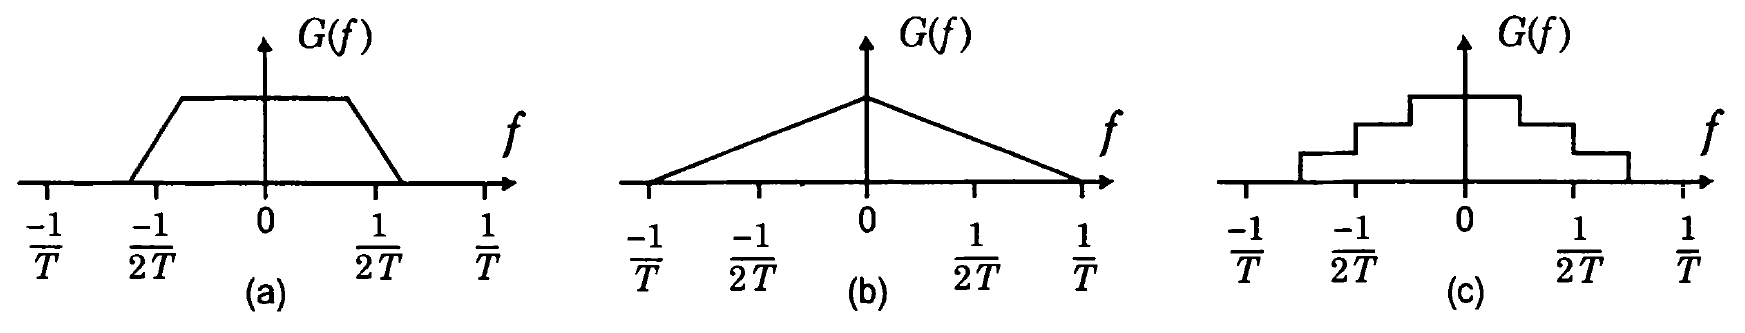
\includegraphics[width=0.8\columnwidth]{figs/pam_07}
	  \end{center}
	\end{figure}
\end{frame}

\begin{frame}
	\frametitle{Impacto da filtragem sobre o PAM}

	\begin{itemize}
	    \item Consideremos agora o impacto do canal, modelado como um filtro linear invariante no tempo com resposta ao impulso $b(t)$ e ruído aditivo $n(t)$.
	\end{itemize}	
	\begin{figure}[t]	
	  \begin{center}
	    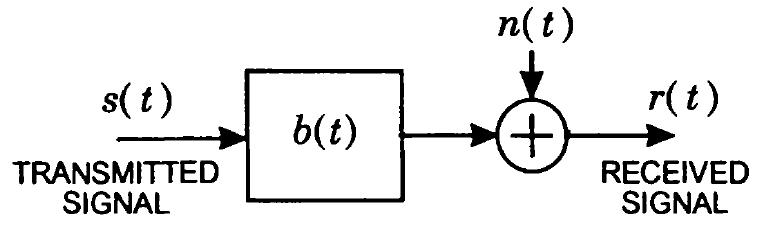
\includegraphics[width=0.4\columnwidth]{figs/pam_08}
	  \end{center}
	\end{figure}
	\begin{itemize}
	    \item Aplicando o sinal PAM nesse modelo obtemos:
	    \begin{align*}
		r(t) = \int_{-\infty}^{\infty}b(\tau)\sum\limits_{m=-\infty}^{\infty} a_m g(t-mT-\tau)d\tau + n(t)
	    \end{align*}
	    \item Para $h(t) = b(t)*g(t)$, chamado de pulso recebido, obtemos
	    \begin{equation*}
		r(t) = \sum\limits_{m=-\infty}^{\infty} a_m h(t-mT) + n(t)
	    \end{equation*}
	\end{itemize}	
\end{frame}

\begin{frame}
	\frametitle{Impacto da filtragem sobre o PAM}

	\begin{itemize}
	    \item Se o sinal transmitido é PAM, o sinal recebido também é PAM, mas com um diferente formato de pulso e com a adição de ruído.
	    \item Filtro de recepção:
	    \begin{itemize}
		\item Compensação da distorção do canal.
		\item Diminuição do efeito do ruído aditivo.
		\item Condicionamento do sinal recebido antes da amostragem.
		\item Pode ser projetado para evitar ISI após amostragem.
	    \end{itemize}
	\end{itemize}		
	\begin{figure}[t]	
	  \begin{center}
	    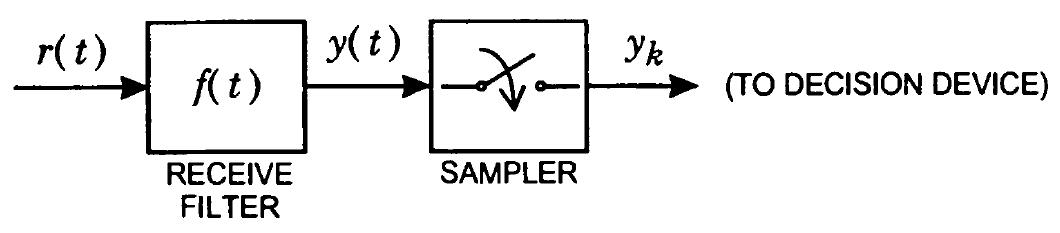
\includegraphics[width=0.6\columnwidth]{figs/pam_09}
	  \end{center}
	\end{figure}
\end{frame}

\begin{frame}
	\frametitle{Impacto da filtragem sobre o PAM}

	\begin{itemize}
	    \item Saída do filtro de recepção antes da amostragem:
	    \begin{equation*}
		y(t) = \sum\limits_{\infty}^{\infty} a_m p(t-mT) + n'(t)
	    \end{equation*}
	    \item Onde $p(t)$ é o formato de pulso resultante, dado por:
	    \begin{equation*}
		p(t) = g(t) * b(t) * f(t) \quad \xrightarrow{\mathcal{F}} \quad P(f) = G(f)B(f)F(f)
	    \end{equation*}
	    \item Para evitar ISI, o pulso resultante deve ser Nyquist, e não somente $g(t)$, portanto:
	    \begin{equation*}
		    p(kt) = \delta_k \quad \xrightarrow{\mathcal{F}} \quad \sum\limits_{m=-\infty}^{\infty} P\left(f-\frac{m}{T} \right) = T
	    \end{equation*}
	\end{itemize}		
\end{frame}

\begin{frame}
	\frametitle{ISI e Diagramas de olho}

	\begin{itemize}
	    \item Cancelamento perfeito da ISI é difícil de ser alcançado:
	    \begin{itemize}
		\item Imperfeições na estimativa de canal.
		\item Limitações práticas de implementação do pulso de transmissão.
	    \end{itemize}
	    \item Diagrama de olho:
	    \begin{itemize}
		\item Ilustra a degradação do sinal.
		\item Pode ser gerado em osciloscópio.
		\item Ferramenta de auxílio na etapa de projeto do sistema.
		\item Consiste da superposição de várias pequenas partes de um sinal.
	    \end{itemize}
	    \item A presença de ISI tende a fechar o olho verticalmente.
	    \item Instante ideal de amostragem é o ponto de máxima abertura.
	    \item Abertura horizontal é importante para reduzir o impacto de erros de temporização.
	\end{itemize}		
\end{frame}

\begin{frame}
	\frametitle{ISI e Diagramas de olho}

	\begin{itemize}
	 \item PAM binário com 50\% de banda excedente.
	\end{itemize}	
	\begin{figure}[t]	
	  \begin{center}
	    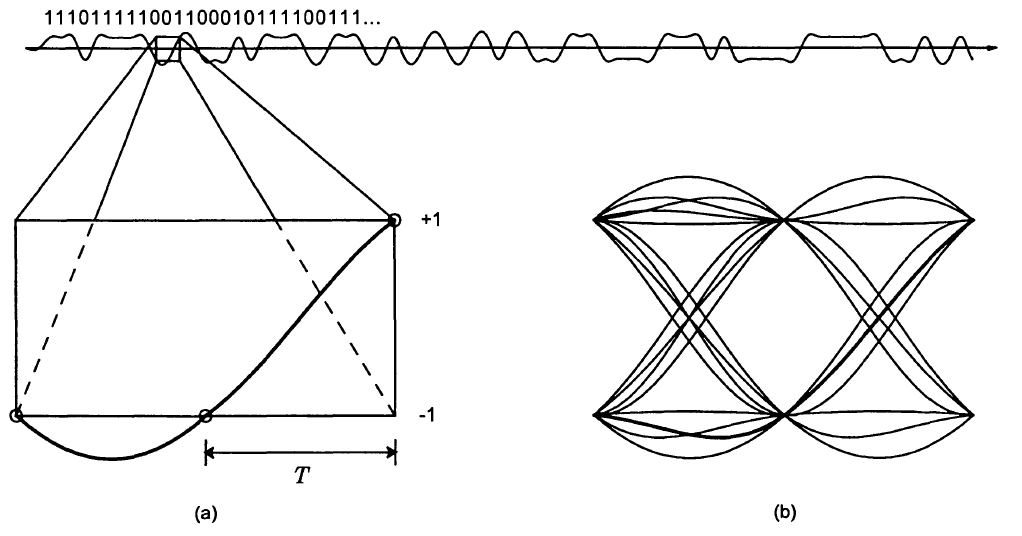
\includegraphics[width=0.9\columnwidth]{figs/pam_10}
	  \end{center}
	\end{figure}
\end{frame}

\begin{frame}
	\frametitle{ISI e Diagramas de olho}

	\begin{columns}	
	    \begin{column}{0.5\textwidth}
		\begin{figure}[t]	
		    \begin{center}
			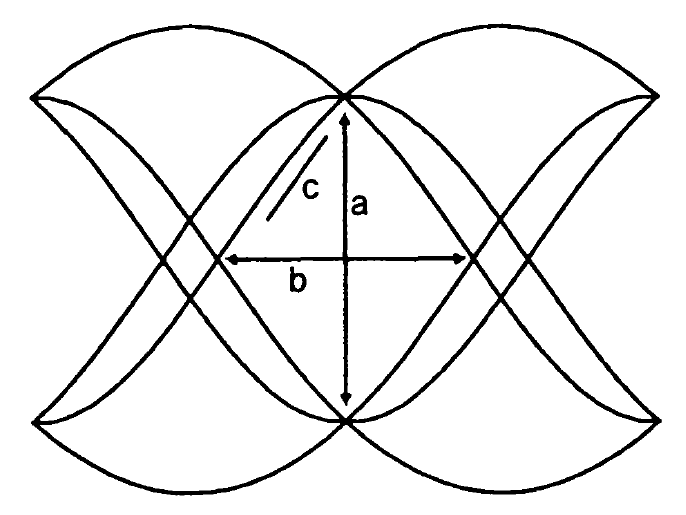
\includegraphics[width=0.8\columnwidth]{figs/pam_11}
		    \end{center}
		\end{figure}
	    \end{column}

	    \begin{column}{0.5\textwidth}
		\begin{enumerate}[a)]
		    \item Abertura vertical indica imunidade a ruído
		    \item Abertura horizontal indica imunidade a erros de temporização.
		    \item Inclinação da pálpebra interna indica a sensibilidade a \textit{jitter} de temporização.
		\end{enumerate}		 
	    \end{column}	
	\end{columns}

\end{frame}

\begin{frame}
	\frametitle{ISI e Diagramas de olho}

	\begin{itemize}
	 \item Diagramas de olho para (a) 25\% e (b) 100\% de banda excedente.
	\end{itemize}	
	
	\begin{figure}[t]	
	  \begin{center}
	    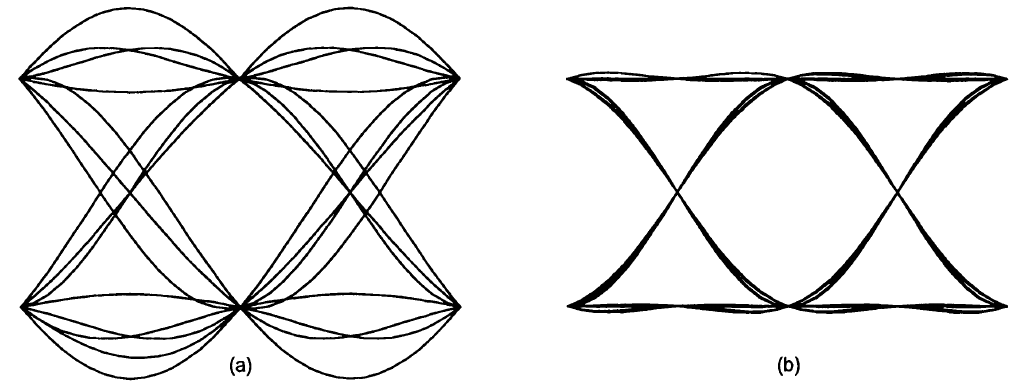
\includegraphics[width=0.9\columnwidth]{figs/pam_12}
	  \end{center}
	\end{figure}
\end{frame}

\begin{frame}
	\frametitle{Taxa de bits e eficiência espectral}

	\begin{itemize}
	  \item Os símbolos são escolhidos, de forma independente e uniforme, do alfabeto $\mathcal{A}$, de tamanho $|\mathcal{A}|$.
	  \item Cada símbolo carrega $\log_2 |\mathcal{A}|$ bits de informação.
	  \item Taxa de bits do PAM:
	  \begin{equation*}
	    R_b = \frac{\log_2 |\mathcal{A}|}{T} \quad \text{ bit/s}
	  \end{equation*}
	  \item Formas de aumentar a taxa:
	  \begin{itemize}
	    \item Aumentar a ordem da modulação (limitação de potência e impacto do ruído)
	    \item Aumentar a taxa de símbolos $1/T$ (limitação de banda e impacto da ISI)
	  \end{itemize}
	  \item Eficiência espectral:
	  \begin{equation*}
	      \nu = \frac{\text{taxa de bits}}{\text{banda}} = \frac{R_b}{W} \quad \text{bit/s/Hz}
	  \end{equation*}
	\end{itemize}	
\end{frame}

\begin{frame}
	\frametitle{Taxa de bits e eficiência espectral}

	\begin{itemize}
	  \item Para o PAM temos: $W=(1+\alpha)/(2T)$
	  \item A eficiência espectral pode ser simplificada para:
	  \begin{equation*}
	      \nu = \frac{R_b}{W} = \frac{\log_2 |\mathcal{A}| / T}{(1+\alpha)/(2T)} = \frac{2\log_2 |\mathcal{A}|}{1+\alpha}
	  \end{equation*}
	  \item Também podemos isolar o tamanho do alfabeto:
	  \begin{equation*}
	      |\mathcal{A}| = 2^{(1+\alpha)\nu / 2}
	  \end{equation*}
	  \item Para o caso do filtro ideal com $\alpha=0$, temos:
	  \begin{equation*}
	      \nu_{\text{max}} = 2 \log_2 |\mathcal{A}| \quad \text{e} \quad |\mathcal{A}| =  2^{\nu_{\text{max}} / 2}
	  \end{equation*}  

	\end{itemize}	
\end{frame}


\section{PAM em banda passante}

\begin{frame}
	\frametitle{Representação em banda passante do PAM}

	\begin{itemize}
	  \item Comunicações práticas normalmente ocorrem em banda passante.
	  \begin{figure}[t]	
	    \begin{center}
	      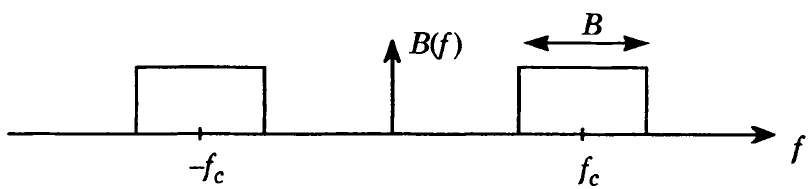
\includegraphics[width=0.6\columnwidth]{figs/pam_13}
	    \end{center}
	  \end{figure}
	  \item Representações em banda passante do PAM:
	  \begin{itemize}
	    \item PAM \textit{double-sideband} (PAM-DSB)
	    \item PAM \textit{single-sideband} (PAM-SSB)
	    \item PAM \textit{em banda passante}
	  \end{itemize}
	\end{itemize}
\end{frame}

\begin{frame}
	\frametitle{PAM-DSB}

	\begin{itemize}
	  \item PAM-DSB modula diretamente o sinal PAM aplicando oscilador local:
	  \begin{equation*}
	      s(t) = \sqrt{2} \cos(2\pi f_c t) \sum_k a_k g(t-kT)
	  \end{equation*}
	  \item Sinal PAM de banda $B/2$ passa a ocupar $B$ em banda passante.
	  \item Aplicando o critério de Nyquist:
	  \begin{equation*}
	      \frac{1}{2T} \leq (B/2) \quad \Longrightarrow \quad \frac{1}{T} \leq B
	  \end{equation*}
	  \item Desta forma a eficiência espectral cai para a metade da eficiência do PAM em banda base:
	  \begin{equation*}
	      \nu_{\text{max}}^{\text{DSB}} = \frac{R_b}{B} = \frac{\log_2 |\mathcal{A}|/T}{1/T} = \log_2 |\mathcal{A}|
	  \end{equation*}
	\end{itemize}
\end{frame}

\begin{frame}
	\frametitle{PAM-SSB}

	\begin{itemize}
	  \item PAM-SSB evita a redundância das faixas laterais, transmitindo somente uma das faixas.
	  \item Pode ser implementado usando um divisor de fase:
	  \begin{figure}[t]	
	    \begin{center}
	      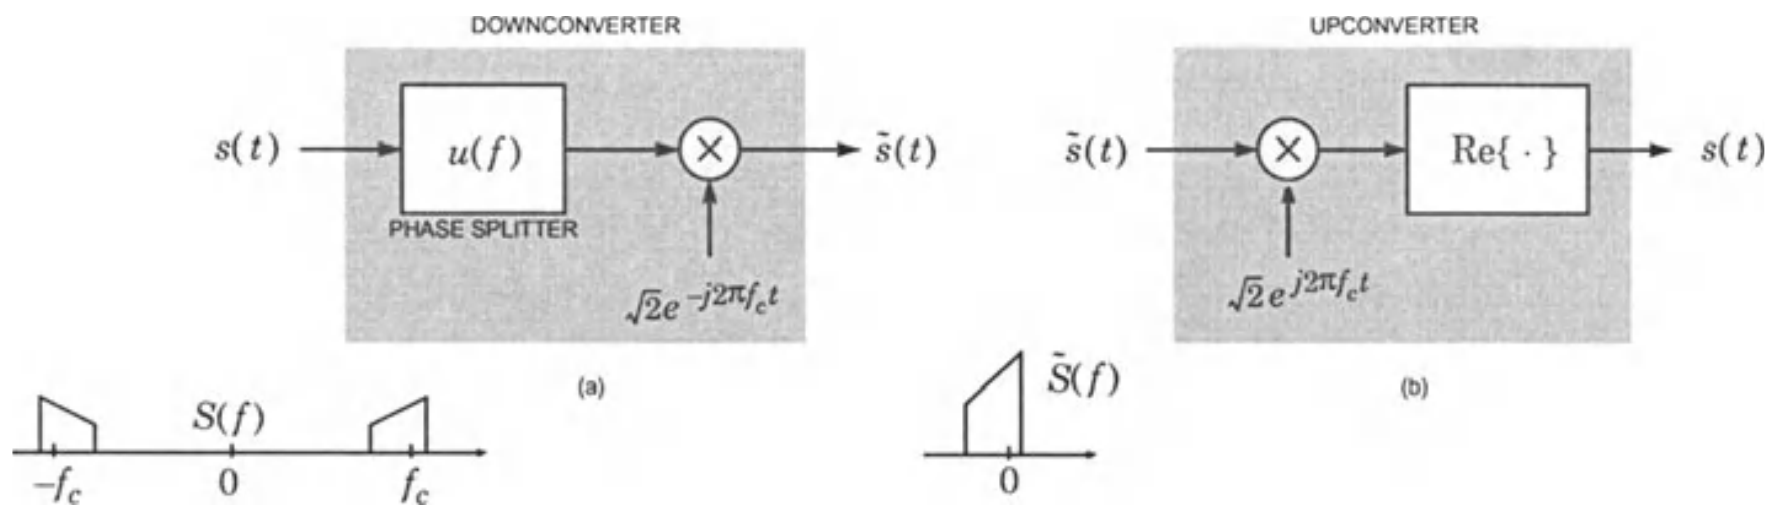
\includegraphics[width=0.9\columnwidth]{figs/pam_22}
	    \end{center}
	  \end{figure}
	  \item Mesma eficiência do PAM em banda base.
	  \item Dificuldade prática de implementação.
	\end{itemize}
	
\end{frame}

\begin{frame}
	\frametitle{PAM em banda passante}

	\begin{itemize}
	  \item Modificação do PAM-DSB para aumentar sua eficiência.
	  \item Definição de componentes em fase $\{ a_k^I \}$ e quadratura $\{ a_k^Q \}$.
	  \begin{equation*}
	      s(t) = \sqrt{2} \cos(2\pi f_c t) \sum_k a_k^I g(t-kT) - \sqrt{2} \sin(2\pi f_c t) \sum_k a_k^Q g(t-kT)
	  \end{equation*}
	  \item O componente em quadratura representa um recurso extra.
	  \item Mesma banda do PAM-DSB, mas com o dobro da eficiência espectral, pois transporta o dobro de informação.
	  \item Classificação com relação à escolha das sequências $\{ a_k^I \}$ e $\{ a_k^Q \}$:
	  \begin{itemize}
	    \item Escolha independente: QAM (modulação em amplitude e quadratura)
	    \item Escolha conjunta: PAM \textit{em banda passante}.
	  \end{itemize}

	\end{itemize}	
\end{frame}

\begin{frame}
	\frametitle{PAM em banda passante}

	\begin{itemize}
	  \item Diagrama de um transmissor PAM em banda passante:
	    \begin{figure}[t]	
	      \begin{center}
		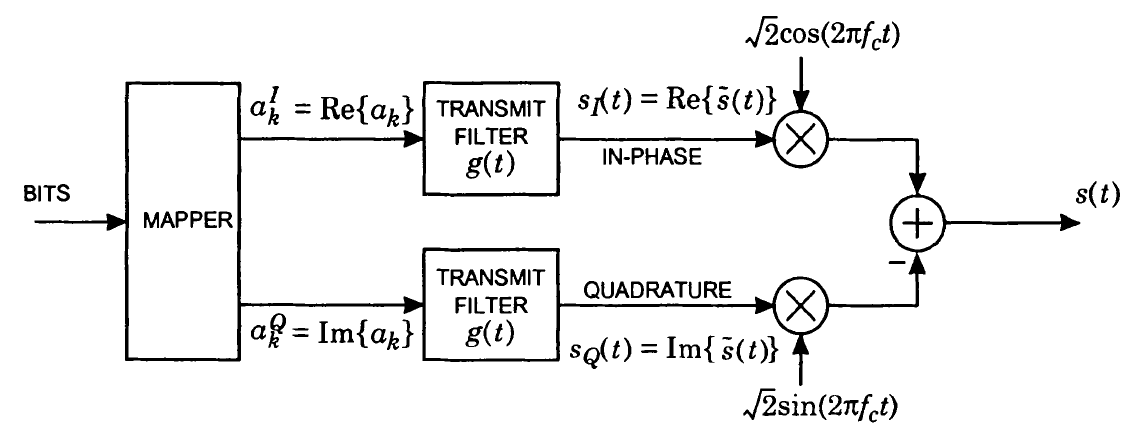
\includegraphics[width=0.9\columnwidth]{figs/pam_14}
	      \end{center}
	    \end{figure}
	\end{itemize}	
\end{frame}

\begin{frame}
	\frametitle{PAM em banda passante}

	\begin{itemize}
	  \item Representação em termos da envoltória complexa:
	  \begin{equation*}
	      s(t) = \sqrt{2} \mathrm{Re}\{ \tilde{s}(t)e^{j2\pi f_c t} \}
	  \end{equation*}
	  \item Onde $\tilde{s}(t)$ corresponde ao equivalente passa-baixa:
	  \begin{equation*}
	      \tilde{s}(t) = \sum_k a_k g(t-kT) \; \text{, com} \quad a_k = a_k^I + j a_k^Q
	  \end{equation*}
	  \item Sinal semelhante ao PAM em banda base, mas com símbolos complexos e pulso real.
	\end{itemize}	
\end{frame}

\begin{frame}
	\frametitle{PAM em banda passante}

	\begin{itemize}
	  \item Implementação alternativa do transmissor PAM baseada na representação complexa:
	    \begin{figure}[t]	
	      \begin{center}
		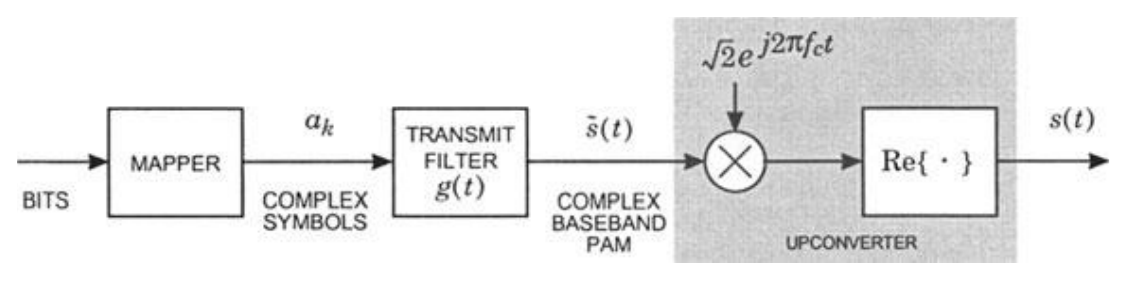
\includegraphics[width=0.75\columnwidth]{figs/pam_15}
	      \end{center}
	    \end{figure}
	   \item Essa implementação é menos eficiente (parte imaginária é computada e descartada), mas a representação complexa é mais compacta e concisa.
	   \item PAM \textit{em banda passante} e SSB duplicam a eficiência do PAM-DSB.
	  \begin{itemize}
	    \item SSB fixa a taxa de bits e corta a banda pela metade.
	    \item PAM \textit{em banda passante} duplica a taxa de bits e mantém a banda.
	  \end{itemize}
	\end{itemize}	
\end{frame}

\begin{frame}
	\frametitle{PAM em banda passante}

	\begin{itemize}
	  \item Representações em: a) fase e quadratura; b) envoltória complexa.
	  \item Terceira representação baseada em coordenadas polares:
	  \begin{align*}
	      a_m &= c_m e^{j \theta_m} \\
	      s(t) &= \sqrt{2} \mathrm{Re} \left\{ \sum_{m=-\infty}^{\infty} c_m e^{j(2\pi f_c t + \theta_m)} g(t-mT) \right\} \\
 	      &= \sqrt{2} \sum_{m=-\infty}^{\infty} c_m \cos(2\pi f_c t + \theta_m) g(t-mT)
	  \end{align*}
	  \item Amplitude e fase da portadora são determinadas por $a_m$.
	  \item Também chamado de AM/PM.
	  \item Indica que o PSK (chaveamento por deslocamento de fase) é um caso particular do PAM em banda passante.
	\end{itemize}	
\end{frame}

\begin{frame}
	\frametitle{Constelações}

	\begin{itemize}
	  \item O alfabeto é o conjunto $\mathcal{A}$ de símbolos disponíveis para transmissão.
	  \item Exemplos:
	  \begin{itemize}
		\item Alfabeto real: $\mathcal{A} = \{ -3. -1, +1, +3 \}$
		\item Alfabeto complexo: $\mathcal{A} = \{ -1. -j, +1, +j \}$
	  \end{itemize}
	    \item Constelação de sinais: conjunto de pontos do alfabeto dispostos em um plano complexo.
	\end{itemize}	
	\begin{figure}[t]	
	      \begin{center}
		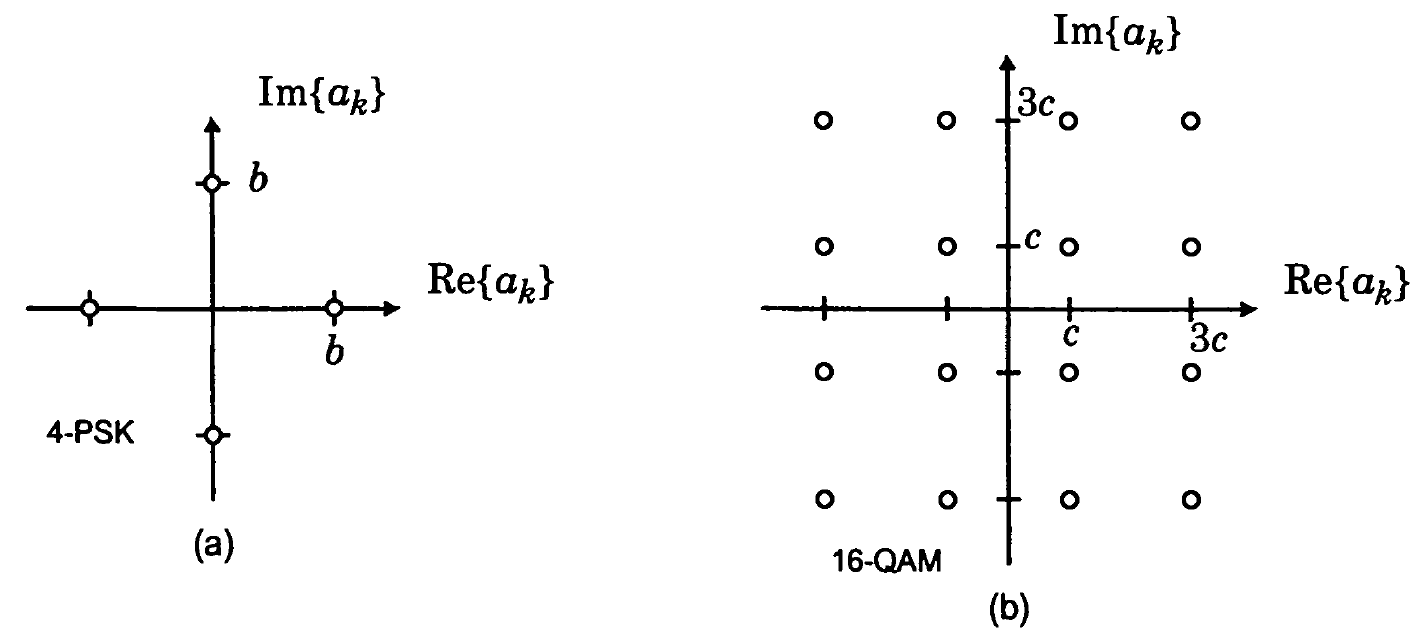
\includegraphics[width=0.7\columnwidth]{figs/pam_17}
	      \end{center}
	    \end{figure}
\end{frame}

\begin{frame}
	\frametitle{Constelações}

	\begin{itemize}
	    \item Cálculo da energia média de um pulso PAM em banda passante.
	    \item Considerações:
	    \begin{itemize}
		\item Símbolos equiprováveis.
		\item Pulso de transmissão $g(t)$ com energia $\mathcal{E}_g$.
		\item Pulso transmitido de forma \textbf{isolada}, por exemplo considerando pulso ideal de Nyquist com zero ISI. Neste caso pode-se omitir o subíndice $k$ relativo ao $k$-ésimo tempo de símbolo, ou seja, $\tilde{s}(t) = a g(t)$.
	    \end{itemize}
	    \item Sinal e seu equivalente passa-baixa: $s(t) = \sqrt{2} \mathrm{Re}\{ \tilde{s}(t) e^{j2\pi f_c t} \}$
	    \item Cálculo da energia média $\mathcal{E}$:
	    \begin{align*}
		\mathcal{E} &= \mathrm{E}\left[ \int_{-\infty}^{\infty} s^2(t) dt \right] = \mathrm{E} \left[ \int_{-\infty}^{\infty} |\tilde{s}(t)|^2 dt \right] = \mathrm{E}[|a|^2]\int_{-\infty}^{\infty} g^2(t) dt \\
		&= \left( \frac{1}{|\mathcal{A}|} \sum_{a \in \mathcal{A}} |a|^2 \right) \int_{-\infty}^{\infty} g^2(t) dt  =  \mathcal{E}_a \mathcal{E}_g
	    \end{align*}
	\end{itemize}	
\end{frame}

\begin{frame}
	\frametitle{Constelações}

	\begin{itemize}
	    \item Considerando a envoltória complexa $\tilde{s}(t)$ do sinal PAM, podemos calcular sua densidade espectral de potência (DEP) $S_{\tilde{s}}(f)$:
	    \begin{equation*}
		S_{\tilde{s}}(f) = \frac{1}{T}|G(f)|^2 S_{a}(f)
	    \end{equation*}
	    \item Onde $G(f)$ é a transformada de Fourier do pulso e $S_a(f)$ é a DEP da sequência de informação.
	    \item Para o caso em que a sequência é branca, a sua DEP é constante, dada por $S_a(f) = \mathcal{E}_a.$
	    \item A potência $P$ pode ser calculada ao integrar a DEP na frequência, obtendo portanto:
	    \begin{equation*}
		P = \int_{-\infty}^{\infty} \frac{1}{T} |G(f)|^2 S_a(f) df = \frac{\mathcal{E}_a}{T}\int_{-\infty}^{\infty} |G(f)|^2 df = \frac{\mathcal{E}_a\mathcal{E}_g}{T} = \frac{\mathcal{E}}{T}
	    \end{equation*}

	\end{itemize}	
\end{frame}

\begin{frame}
	\frametitle{Projeto da constelação}

	\begin{itemize}
	    \item A distância mínima $d_{\text{min}}$ é um parâmetro importante.
	    \item Quanto maior a distância mínima maior a imunidade ao ruído.
	    \item Relação custo-benefício entre potência de transmissão, tamanho da constelação e imunidade ao ruído.
	    \item Projeto da constelação:
	    \begin{itemize}
	      \item Objetivo: maximizar a distância entre símbolos evitando exceder a restrição de potência de transmissão.
	      \item Constelações ótimas podem ser difíceis de derivar e de alto custo.
	      \item Seu \textbf{desempenho} é invariante à translação.
	      \item Qual translação resulta em mínima potência?
	      \begin{equation*}
		\mathrm{E}[|a-m|^2] = \sum_{i=1}^M p_a(a_i) |a_i-m|^2
	      \end{equation*}
	      \item Melhor escolha para translação: $m = \mathrm{E}[a]$.
	      \item Constelação com média zero gasta menos energia que outras translações.
	    \end{itemize}	    	    
	\end{itemize}	
\end{frame}

\begin{frame}
	\frametitle{Projeto da constelação}

	\begin{itemize}
	    \item Exemplos de constelações QAM quadradas ($M=L^2$):
	    \begin{figure}[t]	
	    \begin{center}
	      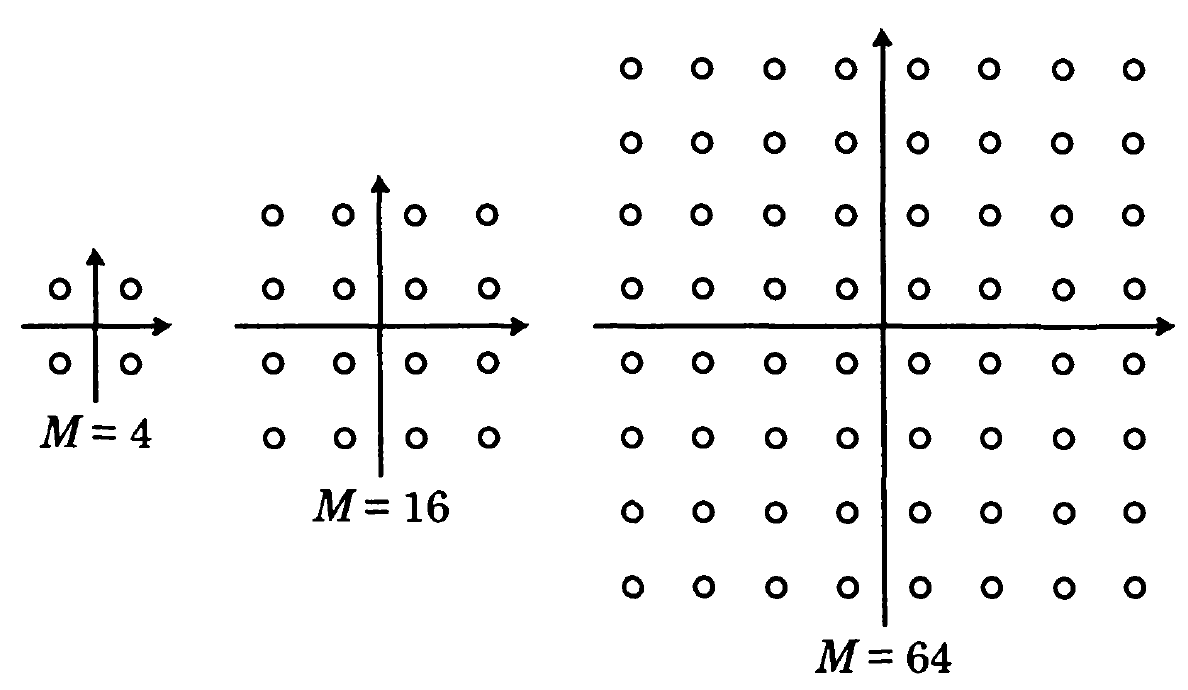
\includegraphics[width=0.45\columnwidth]{figs/pam_18}
	    \end{center}
	  \end{figure}
	    \item Componentes $a_I$ e $a_Q$ são escolhidas de um alfabeto PAM $L$-ário $\{ \pm c, \pm 3c, \ldots, \pm (L-1)c \}$, com $m$-ésimo elemento $c(-L+1+2m)$.
	    \item Energia média de uma constelação $M$-QAM:
	    \small
	    \begin{align*}
		  \mathcal{E}_a &= \mathrm{E}[|a|^2] = \mathrm{E}[a_I^2] + \mathrm{E}[a_I^2] = 2 \mathrm{E}[a_I^2] \\
		  &= \frac{2}{L}\sum_{m=0}^{L-1} c^2(-L+1+2m)^2 = \frac{2}{3}c^2(L^2-1) = \frac{2}{3}c^2(M-1)
	    \end{align*}
	\end{itemize}	
\end{frame}

\begin{frame}
	\frametitle{Projeto da constelação}

	\begin{itemize}
	    \item Exemplos de constelações QAM retangulares ($M\neq L^2$):
	    \begin{figure}[t]	
	    \begin{center}
	      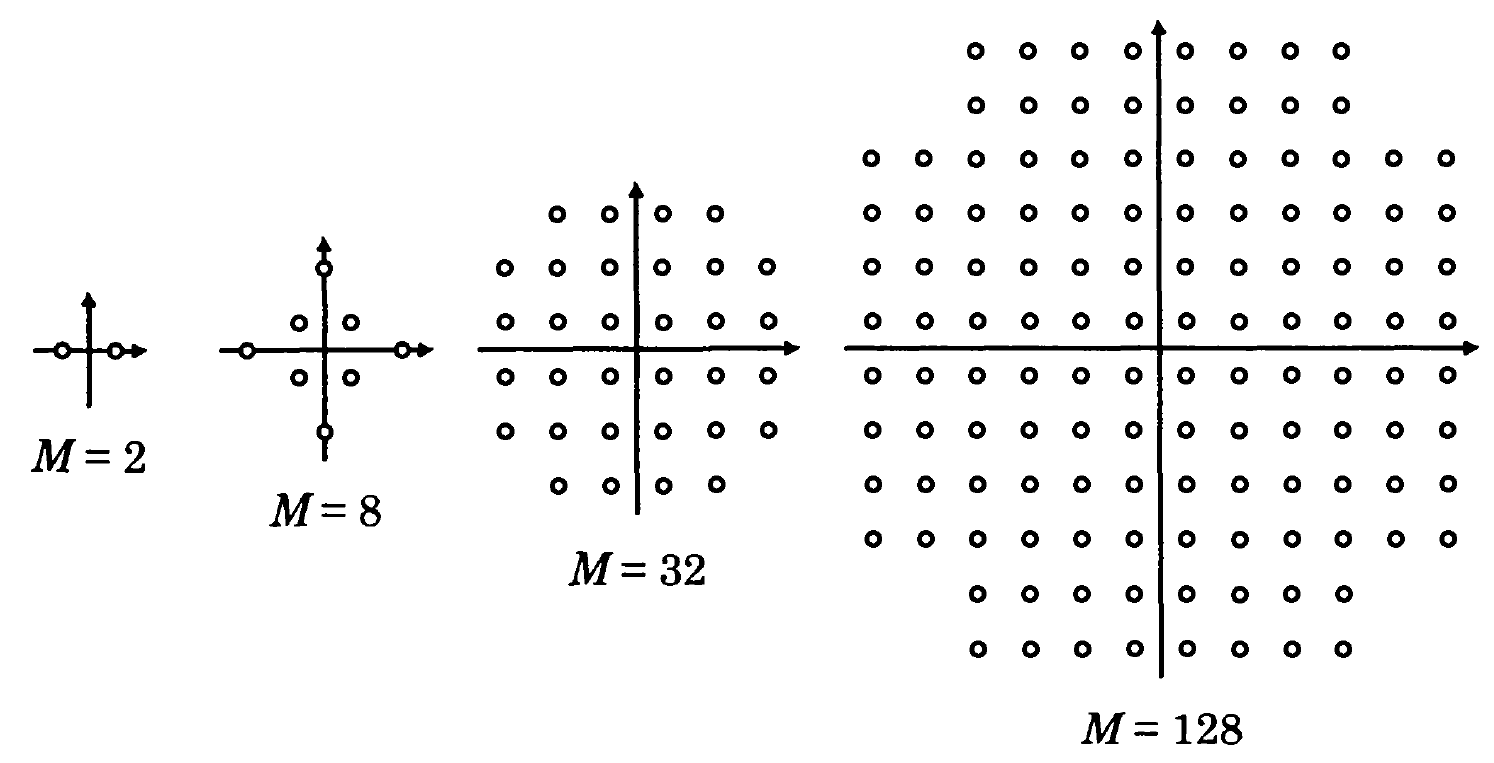
\includegraphics[width=0.55\columnwidth]{figs/pam_19}
	    \end{center}
	  \end{figure}
	    \item Mapeamento ligeiramente mais complicado.
	    \item Aplicações em combinação com códigos em treliça.
	\end{itemize}	
\end{frame}

\begin{frame}
	\frametitle{Projeto da constelação}

	\begin{itemize}
	    \item Exemplos de constelações PSK e AM-PM:
	    \begin{figure}[t]	
	    \begin{center}
	      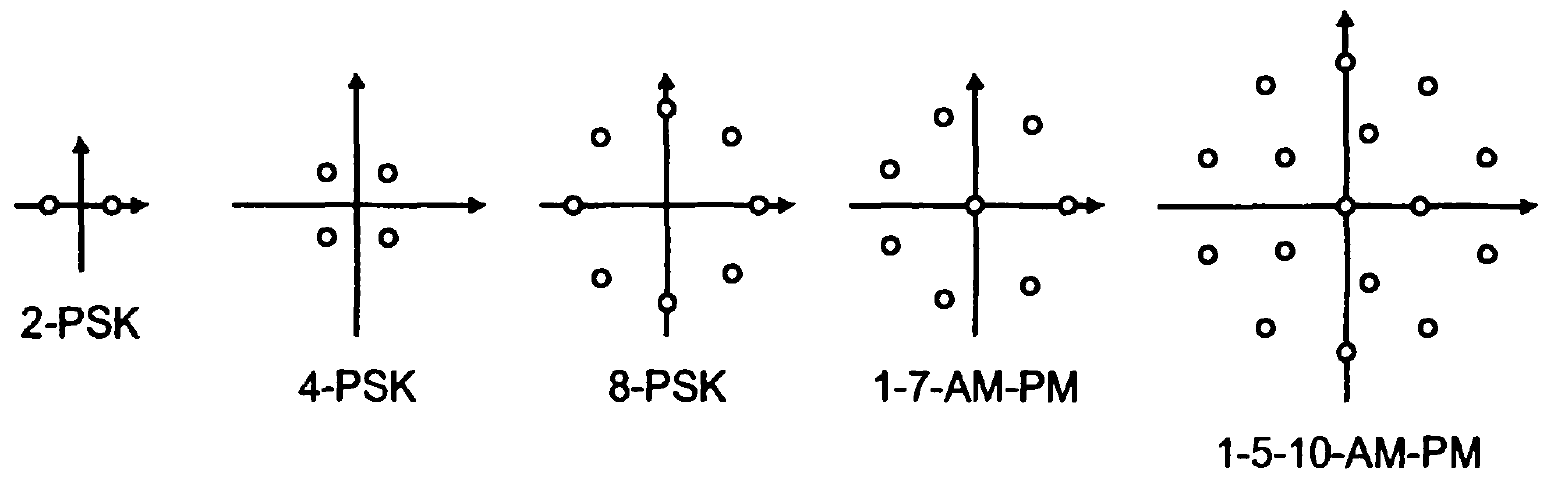
\includegraphics[width=0.7\columnwidth]{figs/pam_20}
	    \end{center}
	  \end{figure}
	    \item Elementos do alfabeto PSK: $a = \sqrt{\mathcal{E}} e^{j2\pi m/M}$
	    \item Envoltória constante e pontos com mesma energia.
	    \item Implementação de receptor de baixo custo.
	\end{itemize}	
\end{frame}

\begin{frame}
	\frametitle{Projeto da constelação}

	\begin{itemize}
	    \item Exemplos de constelações hexagonais:
	    \begin{figure}[t]	
	    \begin{center}
	      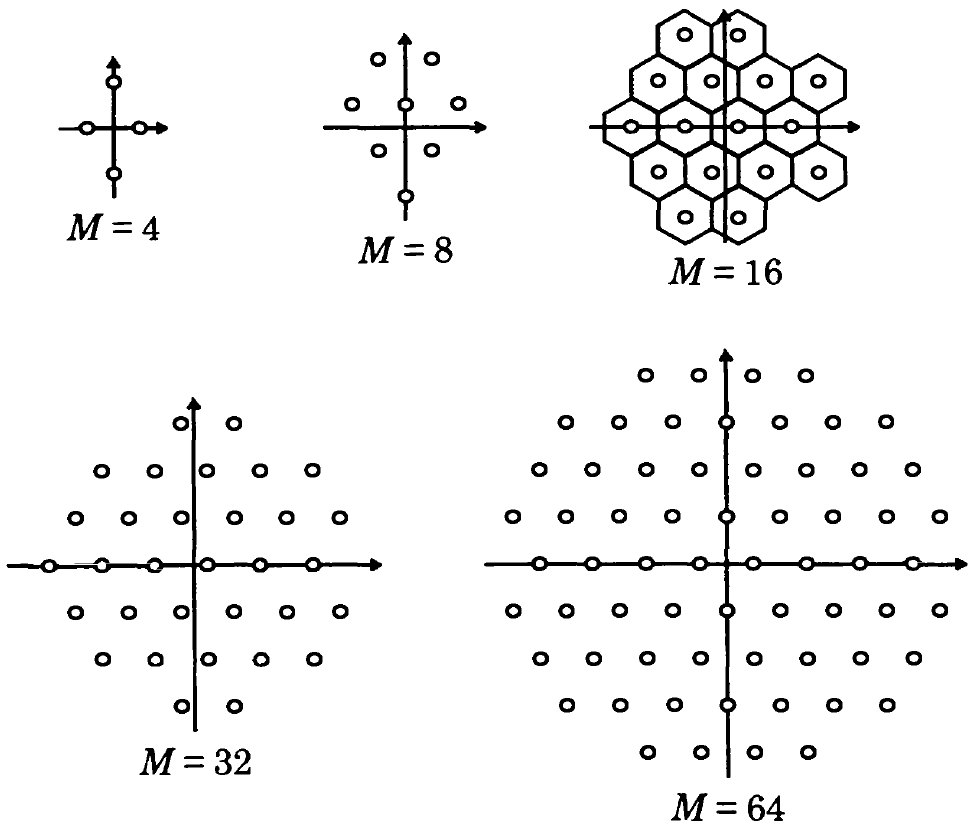
\includegraphics[width=0.45\columnwidth]{figs/pam_21}
	    \end{center}
	  \end{figure}
	    \item Símbolos localizados nos vértices de triângulos equiláteros.
	    \item Regiões de decisão hexagonais.
	    \item Desempenho ligeiramente superior a constelações retangulares, mas com complexidade elevada.
	\end{itemize}	
\end{frame}

\section{Receptor de distância mínima}

\begin{frame}
	\frametitle{Critério de distância mínima}

	\begin{itemize}
	    \item Mudamos agora o foco para o projeto do receptor.
	    \item Vamos considerar inicialmente a ausência de ISI, ou seja, assumindo que somente um pulso  é transmitido.
	    \item Projeto baseado em distância mínima e estrutura do filtro casado.
	    \item Expressão do sinal recebido considerando a transmissão de um único símbolo $a \in \mathcal{A}$:
	    \begin{equation*}
		r(t) = ah(t) + n(t)
	    \end{equation*}
	    \item Onde $h(t)$ é o pulso recebido e $n(t)$ é o ruído.
	    \item Modelo aplicável ao PAM em banda base ou em banda passante (foco no último caso, que é mais geral).
	    \item \textcolor{red}{Problema}: determinar a partir de $r(t)$ qual símbolo foi transmitido.
	\end{itemize}	
\end{frame}

\begin{frame}
	\frametitle{Critério de distância mínima}

	\begin{itemize}
	    \item Exemplo considerando sinalização binária antipodal, $\mathcal{A} = \{ -1, +1 \}$. 
	    \item Sina recebido sem ruído: $h(t)$ ou $-h(t)$
	\end{itemize}	
	\begin{columns}
		\begin{column}{0.5\textwidth}
		    \begin{figure}[t]	
		      \begin{center}
			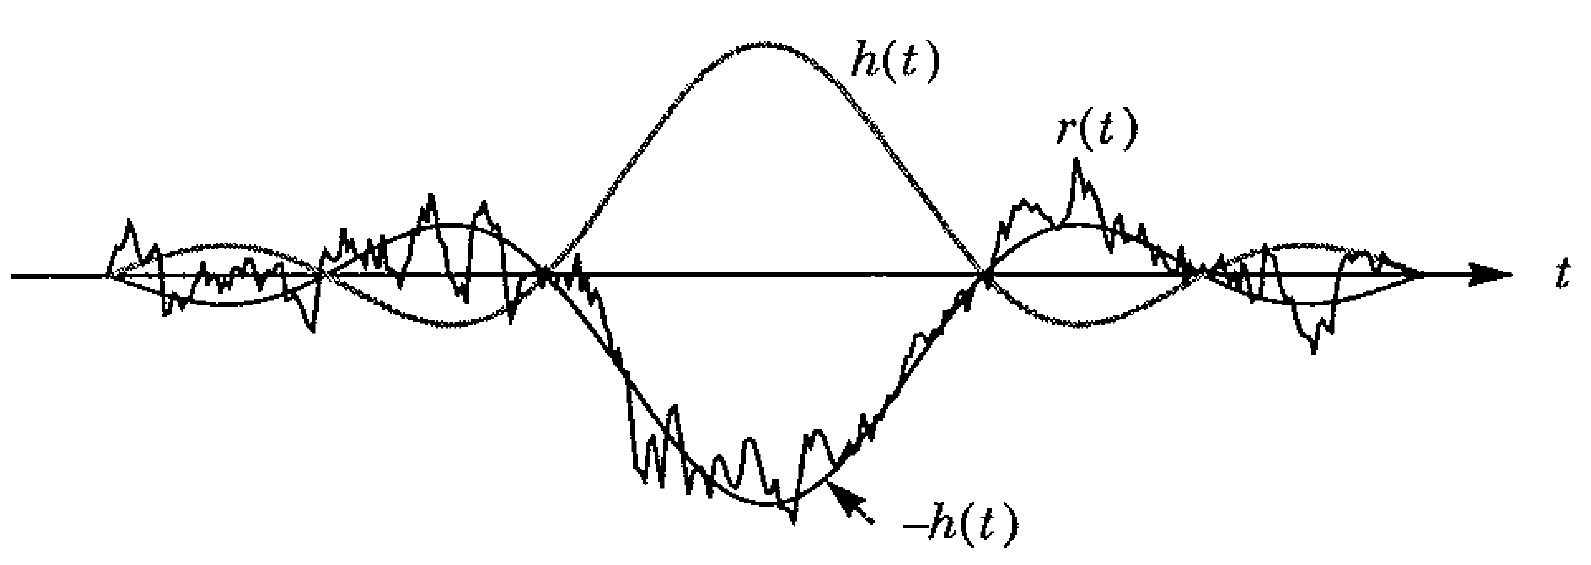
\includegraphics[width=\columnwidth]{figs/pam_23}
		      \end{center}\vspace{0.5cm}
		      \caption{Sinais antipodais e sinal recebido, dado que $-1$ foi transmitido.}
		    \end{figure}
		\end{column}
		\begin{column}{0.5\textwidth}
		     \begin{figure}[t]	
		      \begin{center}
			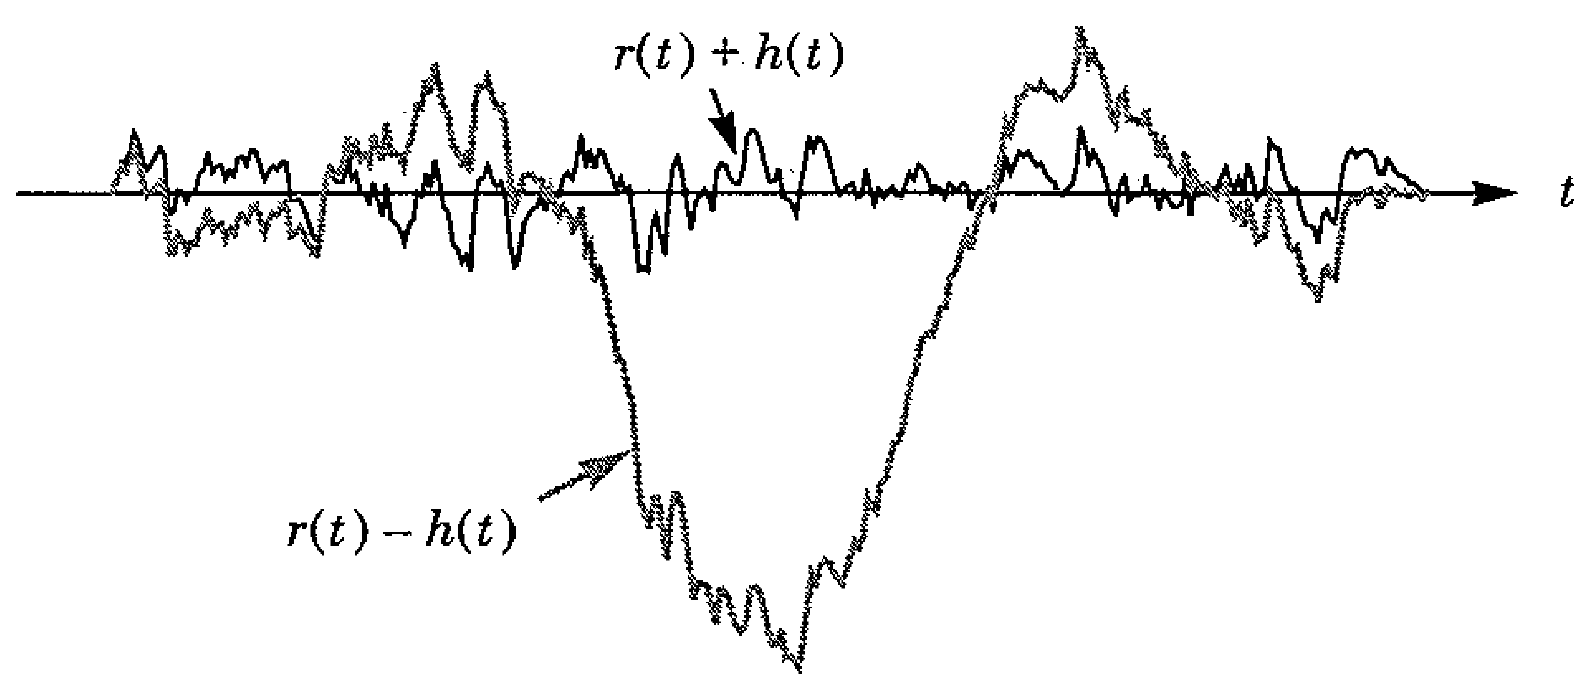
\includegraphics[width=\columnwidth]{figs/pam_24}
		      \end{center}
		      \caption{Diferença entre o sinal recebido e cada um dos sinais da constelação.}
		    \end{figure}
		\end{column}
	\end{columns}
	
\end{frame}

\begin{frame}
	\frametitle{Critério de distância mínima}

	\begin{itemize}
	    \item Quanto menor a diferença entre o sinal recebido e uma dada forma de onda, mais provável que esta tenha sido transmitida.
	    \item Essa métrica pode ser expressa como a energia do sinal da diferença:
	    \begin{equation*}
		\int_{-\infty}^{\infty} |r(t) -h(t)|^2 dt \quad \text{e} \quad \int_{-\infty}^{\infty} |r(t) +h(t)|^2 dt
	    \end{equation*}
	    \item O resultado é comparado e decide por $\hat{a}=1$ se a primeira energia for menor, ou por  $\hat{a}=-1$ se a segunda for menor.
	    \item De forma geral o \textbf{receptor de mínima distância} resolve o problema:
	    \begin{equation*}
		\hat{a} = \arg\min_{a\in \mathcal{A}} \int_{-\infty}^{\infty} |r(t) - ah(t)|^2 dt
	    \end{equation*}

	\end{itemize}			
\end{frame}

\begin{frame}
	\frametitle{Critério de distância mínima}

	\begin{itemize}
	    \item Análise da função custo $J$:
	    \begin{align*}
		J &= \int_{-\infty}^{\infty} |r(t) - ah(t)|^2 dt \\ &= \underbrace{\int_{-\infty}^{\infty} |r(t)|^2 dt}_{\mathcal{E}_r} - 2\mathrm{Re}\biggl\{ a^* \underbrace{\int_{-\infty}^{\infty} r(t)h^*(t) dt}_{y \, (\text{correlação})} \biggr\} + |a|^2 \underbrace{\int_{-\infty}^{\infty} |h(t)|^2 dt}_{\mathcal{E}_h}
% 		&=  - 2\mathrm{Re}\{ a^* y \} + |a|^2 \mathcal{E}_h
	    \end{align*}
	    \item Minimizar a distância equivale portanto a maximizar a correlação:
	    \begin{equation*}
		\hat{a} = \arg\max_{a\in \mathcal{A}} \, 2\mathrm{Re}\left\{ a^* \int_{-\infty}^{\infty} r(t) h^*(t) dt \right\} - |a|^2 \mathcal{E}_h
	    \end{equation*}
	    \item Implementação é simplificada, pois basta calcular uma vez a integral.
	\end{itemize}			
\end{frame}

\begin{frame}
	\frametitle{Critério de distância mínima}

	\begin{itemize}
	    \item Possíveis implementações da integral de correlação:
	\end{itemize}	
	\begin{columns}
		\begin{column}{0.45\textwidth}
		    \begin{figure}[t]	
		      \begin{center}
			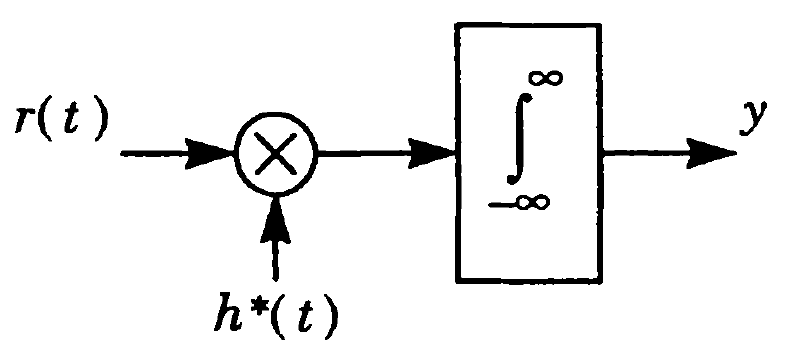
\includegraphics[width=0.75\columnwidth]{figs/pam_25}
		      \end{center}\vspace{-0.1cm}
		      \caption{Correlator.}
		    \end{figure}
		\end{column}
		\begin{column}{0.45\textwidth}
		     \begin{figure}[t]	
		      \begin{center}
			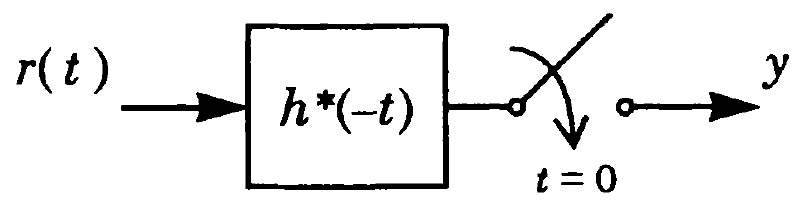
\includegraphics[width=0.85\columnwidth]{figs/pam_26}
		      \end{center}\vspace{0.5cm}
		      \caption{Filtro casado (MF).}
		    \end{figure}
		\end{column}
	\end{columns}
	\begin{itemize}
	    \item O MF é preferível ao correlator, pois permite compensar erros de sincronismo ao ajustar o instante de amostragem.
	\end{itemize}
\end{frame}

\begin{frame}
	\frametitle{Critério de distância mínima}

	\begin{itemize}
	    \item A função custo também pode ser reescrita como:
	    \begin{align*}
		J &= \mathcal{E}_h \left( \frac{\mathcal{E}_r}{\mathcal{E}_h} -2\mathrm{Re} \left\{ a^* \frac{y}{\mathcal{E}_h} \right\} + |a|^2 \right) = \mathcal{E}_h \left| \frac{y}{\mathcal{E}_h} - a  \right|^2 - \frac{|y|^2}{\mathcal{E}_h} + \mathcal{E}_r
	    \end{align*}
	    \item O que leva ao problema equivalente de distância mínima:
	    \begin{equation*}
		\hat{a} = \arg\min_{a \in \mathcal{A}} \left| \frac{y}{\mathcal{E}_h} - a \right|^2
	    \end{equation*}
	    \item Correlação normalizada $z = y / \mathcal{E}_h$
	    \item Decisão: quantização de $z$ para o símbolo mais próximo do alfabeto, também chamado de \textit{slicer}.
	    \begin{figure}[t]	
	    \begin{center}
	      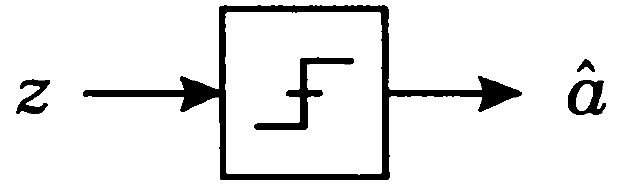
\includegraphics[width=0.25\columnwidth]{figs/pam_27}
	    \end{center} 
	  \end{figure}
	\end{itemize}		
\end{frame}

\begin{frame}
	\frametitle{Critério de distância mínima}

	\begin{itemize}
	    \item Resumo do esquema de recepção do PAM em banda passante:
	    \begin{figure}[t]	
	    \begin{center}
	      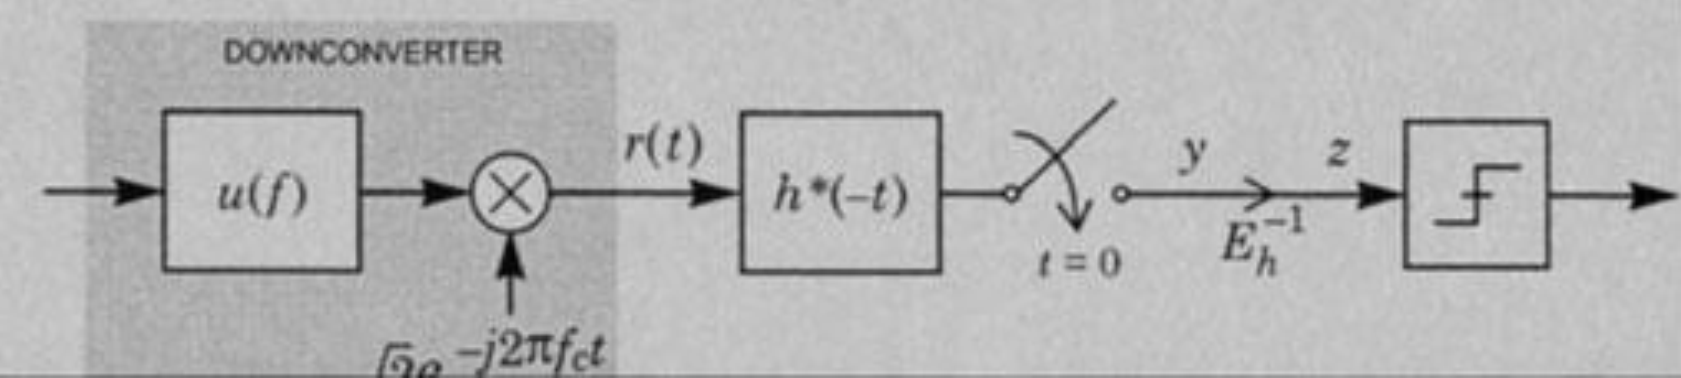
\includegraphics[width=0.8\columnwidth]{figs/pam_28}
	    \end{center} 
	  \end{figure}
	    \item Elementos: translação de frequência, filtro casado, amostragem, quantização (\textit{slicer}).
	    \item Para o PAM em banda base não é necessária a translação de frequência.
	\end{itemize}		
\end{frame}

\begin{frame}
	\frametitle{Propriedades do filtro casado}

	\begin{itemize}
	    \item O filtro casado representa uma forma de implementar o receptor de distância mínima.
	    \item Também pode ser demonstrado que \textcolor{blue}{o MF maximiza a SNR de recepção}.
	    \item Considere um filtro de recepção com resposta ao impulso $f(t)$. Segue a saída do filtro e sua posterior amostragem.
	    \begin{equation*}
		y(t) = \int_{-\infty}^{\infty} r(\tau)f(t-\tau)d\tau \; \xrightarrow{\text{amost. em } \; t=0} y(0) = \int_{-\infty}^{\infty} r(\tau)f(-\tau)d\tau
	    \end{equation*}
	    \item Substituindo $r(t)$ obtemos:
	    \begin{equation*}
		y = \underbrace{a \int_{-\infty}^{\infty} h(t) f(-t) dt}_{\textcolor{blue}{S}} + \underbrace{\int_{-\infty}^{\infty} n(t) f(-t) dt}_{\textcolor{red}{N}}
	    \end{equation*}

	\end{itemize}		
\end{frame}

\begin{frame}
	\frametitle{Propriedades do filtro casado}

	\begin{itemize}
	    \item Definição da relação sinal-ruído (SNR) no receptor:
	    \begin{equation*}
		SNR = \frac{\mathrm{E}[|S|^2]}{\mathrm{E}[|N|^2]} = \frac{\mathrm{E}[|a|^2]\left|\int h(t)f(-t)dt \right|^2}{N_0 \int |f(-t)|^2 dt} = \frac{\mathcal{E}_a \left|\int h(t)f(-t)dt \right|^2}{N_0 \mathcal{E}_f}
	    \end{equation*}
	    \item Considere a desigualdade de Schwarz: 
	    \begin{equation*}
		 \left| \int_{-\infty}^{\infty} u(t) v^*(t) dt \right|^2 \leq \int_{-\infty}^{\infty} |u(t)|^2 dt \int_{-\infty}^{\infty} |v(t)|^2 dt
	    \end{equation*}
	    \item O valor máximo é obtido para $v(t) = K u(t)$, onde $K$ é uma constante.
	    \item Aplicando a desigualdade para o numerador da SNR, obtemos o valor máximo para $f(t) = h^*(-t)$, resultando em
	    \begin{equation*}
		    SNR_{\text{max}} = \frac{\mathcal{E}_a \int |h(t)|^2 dt \int |f(t)|^2dt}{N_0 \mathcal{E}_f} = \frac{\mathcal{E}_a \mathcal{E}_h }{ N_0 }
	    \end{equation*}

	\end{itemize}
\end{frame}

\begin{frame}
	\frametitle{Filtro casado e ISI}

	\begin{itemize}
	    \item A otimização anterior desconsiderou o efeito da ISI.
	    \item A transmissão de uma sequência de pulsos geralmente introduz ISI.
	    \item Excessão para o caso em que o formato do pulso resultante obedece o critério de Nyquist.
	    \item A saída do filtro casado $h^*(-t)$ possui resposta em frequência $|H(f)|^2$.
	    \item O critério de Nyquist pode portanto ser expresso como:
	    \begin{equation*}
		    S_h(f) = \frac{1}{T} \sum_{m=-\infty}^{\infty} \left| H\left(f - \frac{m}{T} \right) \right|^2 = 1
	    \end{equation*}
	    \item O termo $S_h(f)$ é chamado de espectro dobrado (\textit{folded spectrum}) do pulso recebido.
	    \item Para cancelar a ISI pode ser aplicado um filtro de recepção raiz do cosseno levantado:
	    \begin{equation*}
		    H(f) = F(f) = P(f)^{1/2}
	    \end{equation*}

	\end{itemize}
\end{frame}

\begin{frame}
	\frametitle{Receptores PAM em banda passante}

	\begin{itemize}
	    \item Formas alternativas de implementação do PAM em banda passante:
	\end{itemize}
	\begin{figure}[t]	
	    \begin{center}
	    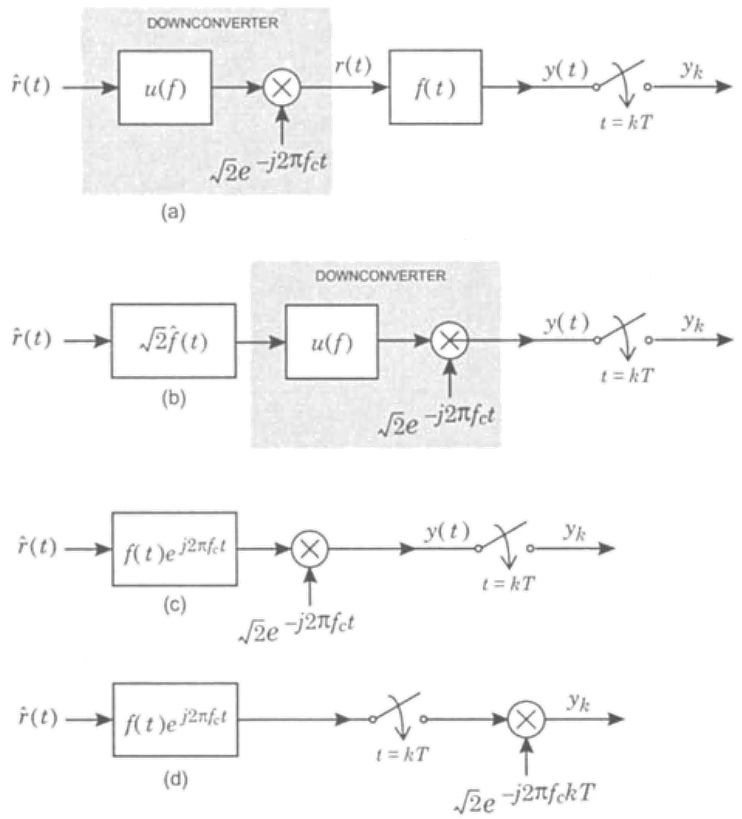
\includegraphics[width=0.5\columnwidth]{figs/pam_29}
	    \end{center} 
	\end{figure}
\end{frame}

\begin{frame}
	\frametitle{Receptores PAM em banda passante}

	\begin{itemize}
	    \item Receptores PAM mais elaborados:
	\end{itemize}
	\begin{figure}[t]	
	    \begin{center}
	    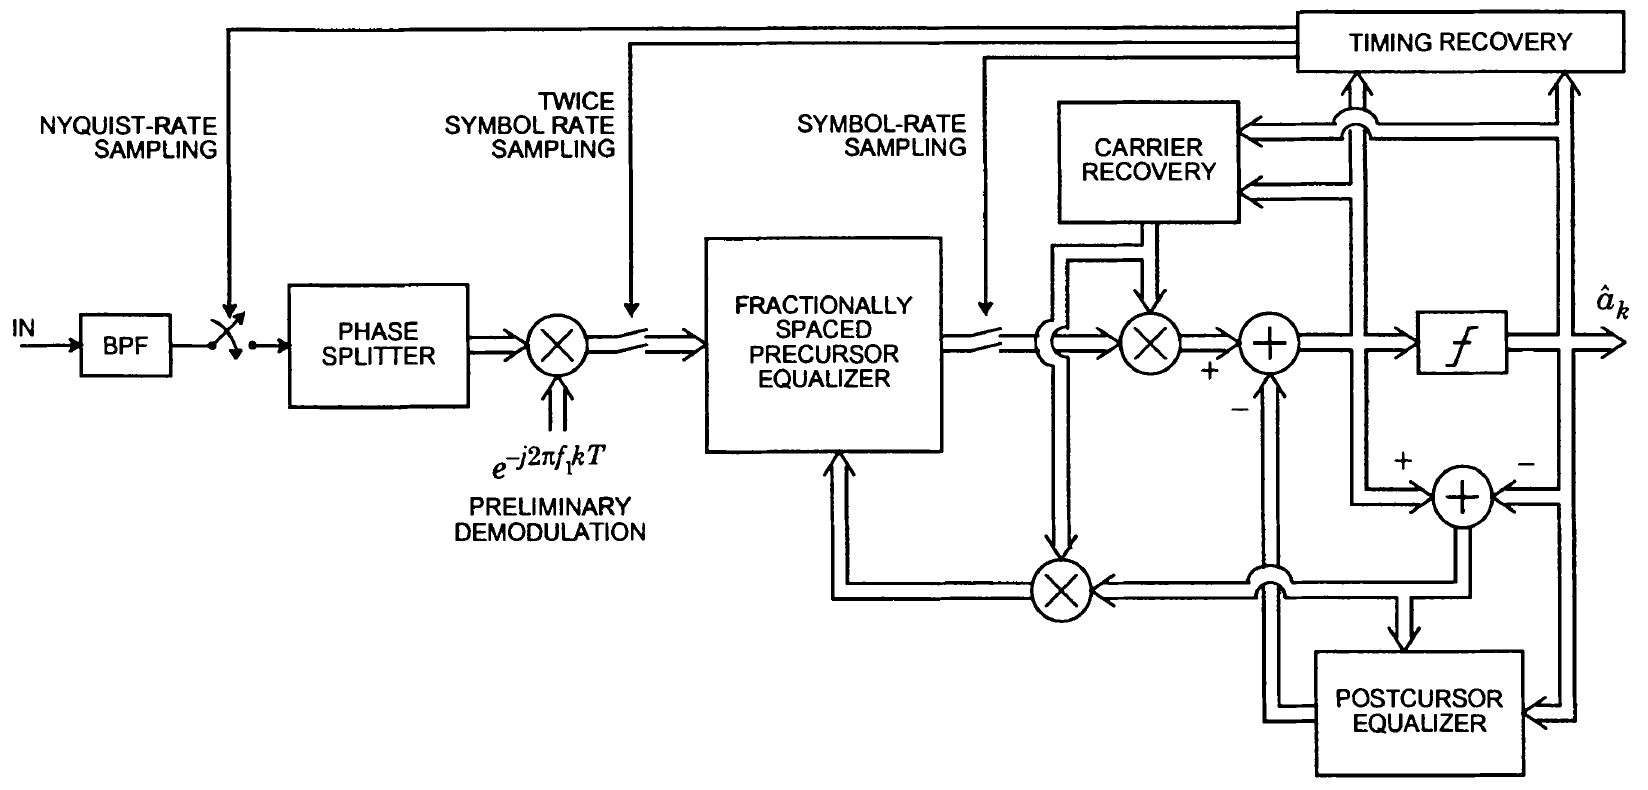
\includegraphics[width=0.9\columnwidth]{figs/pam_30}
	    \end{center} 
	\end{figure}
\end{frame}

\section{Detecção de sequência de distância mínima}

\begin{frame}
	\frametitle{Detecção de sequência de distância mínima}

	\begin{itemize}
	    \item Extensão do conceito de distância mínima para o caso ISI.
	    \item Sequência de $L$ símbolos: $ \mathcal{S} = \{ a_0, a_1, \ldots, a_{L-1} \}$, com $a_i \in \mathcal{A}$ e $M=|\mathcal{A}|$.
	    \item Expressão do sinal recebido:
	    \begin{equation*}
		r(t) = \sum_{k=0}^{L-1} a_k h(t-kT) + n(t)
	    \end{equation*}
	    \item Projeto do detector de sequência de distância mínima:
	    \begin{equation*}
		\hat{\mathcal{S}}_k = \arg \min_{\mathcal{S} \in \mathcal{A}^L} \int_{-\infty}^{\infty} \left| r(t) - \sum_{k=0}^{L-1} a_k h(t-kT) \right|^2 dt
	    \end{equation*}
	    \item Dentre as $M^L$ possíveis sequências, o receptor escolhe aquela que mais se aproxima do sinal observado $r(t)$.
	\end{itemize}	
\end{frame}

\begin{frame}
	\frametitle{Detecção de sequência de distância mínima}

	\begin{itemize}
	    \item A decisão é feita sobre toda a sequência, e não símbolo a símbolo.
	    \item Decisor deve esperar a chegada de todos os símbolos da sequência para tomar a decisão.
	    \item \textcolor{red}{Atraso} na decodificação é proporcional ao tamanho $L$ da sequência.
	    \item Conceito simples, mas \textcolor{red}{complexidade exponencial} em $L$.
	    \item Como tornar a implementação prática?
	\end{itemize}	
\end{frame}

\begin{frame}
	\frametitle{Detecção de sequência de distância mínima}

	\begin{itemize}
	    \item Reescrevendo a função custo:
	\end{itemize}	
	\begin{footnotesize}
	\begin{align*}
	    &J = \int_{-\infty}^{\infty} \left| r(t) - \sum_{k=0}^{L-1} a_k h(t-kT) \right|^2 dt \\
	    &= \mathcal{E}_r - 2\mathrm{Re}\Biggl\{ \sum_{k=0}^{L-1} a_k^* \underbrace{\int_{-\infty}^{\infty} \hspace{-0.15cm} r(t)h^*(t-kT) dt}_{y_k} \Biggr\} + \sum_{k=0}^{L-1} \sum_{j=0}^{L-1} a_k a_j^* \underbrace{\int_{-\infty}^{\infty} \hspace{-0.15cm} h(t-kT)h^*(t-jT) dt}_{\rho_h(j-k)} \\
	    &= \mathcal{E}_r - 2\mathrm{Re}\Biggl\{ \sum_{k=0}^{L-1} a_k^* y_k \Biggr\} + \sum_{k=0}^{L-1} \sum_{j=0}^{L-1} a_k a_j^* \rho_h(j-k)
	\end{align*}
	\end{footnotesize}
	\begin{itemize}
	    \item Problema equivalente a maximizar a correlação:
	    \begin{footnotesize}
	    \begin{equation*}
		\hat{\mathcal{S}}_k = \arg \max_{\mathcal{S} \in \mathcal{A}^L} \; 2\mathrm{Re}\Biggl\{ \sum_{k=0}^{L-1} a_k^* y_k \Biggr\} - \sum_{k=0}^{L-1} \sum_{j=0}^{L-1} a_k a_j^* \rho_h(j-k)
	    \end{equation*}
	    \end{footnotesize}
	\end{itemize}	
\end{frame}

\begin{frame}
	\frametitle{Detecção de sequência de distância mínima}

	\begin{itemize}
	    \item Correlações podem ser calculadas pelo filtro casado amostrado:
	    \begin{figure}[t]	
		\begin{center}
		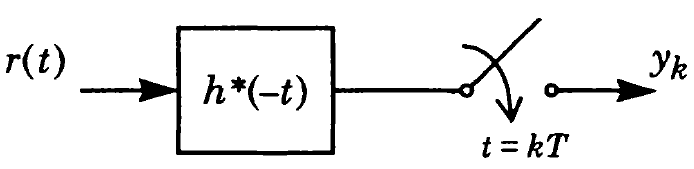
\includegraphics[width=0.35\columnwidth]{figs/pam_31}
		\end{center} 
	    \end{figure}
	    \item Na presença de ISI o filtro casado acentua as distorções de canal.
	    \item Impacto do filtro casado e de equalizador sobre um pulso de recepção que não satisfaz o critério de Nyquist:
	    \begin{figure}[t]	
		\begin{center}
		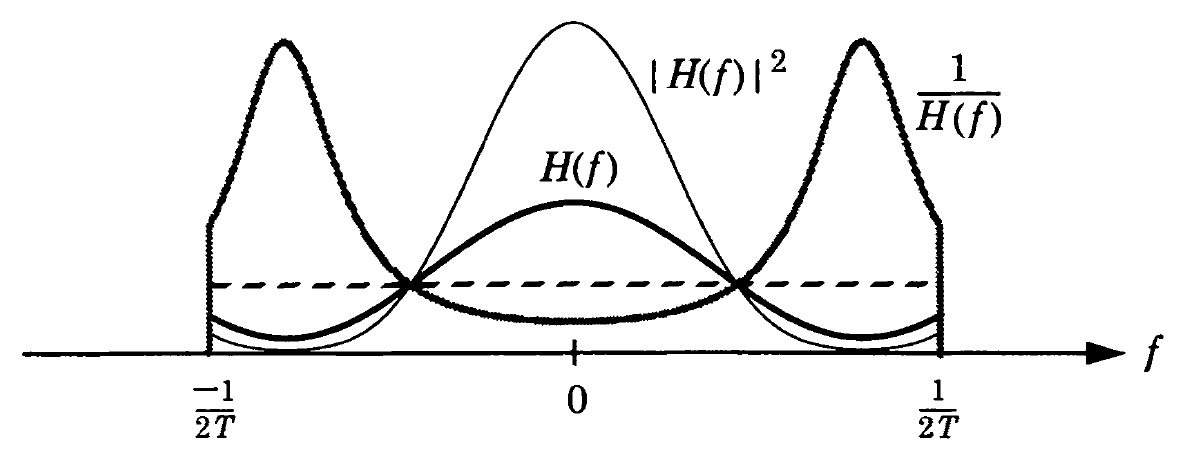
\includegraphics[width=0.5\columnwidth]{figs/pam_32}
		\end{center} 
	    \end{figure}
	    \item Critério da distância mínima maximiza a SNR, mas não evita a ISI.
	\end{itemize}
\end{frame}

\begin{frame}
	\frametitle{Detecção de sequência de distância mínima}

	\begin{itemize}
	    \item Auto-correlação amostrada do pulso recebido: $\rho_h(k) = \langle h(t), h(t-kT) \rangle$
	    \item Propriedades de $\rho_h(k)$:
	    \begin{itemize}
		\item Valor em $k=0$ dado por $\rho_h(0) = \mathcal{E}_h$
		\item Simetria Hermitiana: $\rho_h(-k) = \rho_h^*(k)$
		\item Valor máximo em $\rho_h(0)$, ou seja, $|\rho_h(k)| \leq \rho_h(0) \, , \; \forall k$
		\item Auto-correlação amostrada pode ser vista como a saída de um filtro casado amostrado quando o pulso recebido é a entrada:
	    \end{itemize}
	    \begin{figure}[t]	
		\begin{center}
		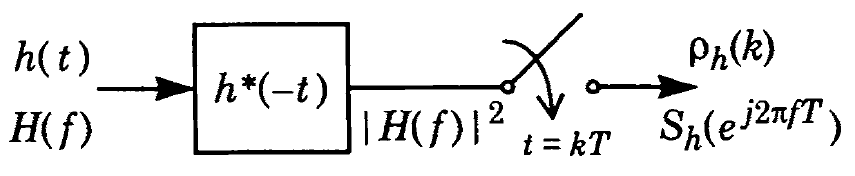
\includegraphics[width=0.4\columnwidth]{figs/pam_33}
		\end{center} 
	    \end{figure}
	    \item Transformada discreta de Fourier da auto-correlação amostrada:
	    \begin{equation*}
		S_h(e^{j2\pi fT}) = \frac{1}{T} \sum_{m=-\infty}^{\infty} | H(f-m/T) |^2
	    \end{equation*}
	    \item Critério de Nyquist: $S_h(e^{j2\pi fT}) = \mathcal{E}_h$ e $\rho_h(k) = \mathcal{E}_h \delta_k$
	\end{itemize}
\end{frame}

\begin{frame}
	\frametitle{Estudo de caso: sinal NRZI}

	\begin{itemize}
	    \item Sinal com memória NRZI: \textit{non-return-to-zero, inverted}
	    \item Codificação diferencial, transições ocorrem quando $1$ é transmistido.
	    \item Sequência codificada de saída $\{b_k \}$, sequência de entrada $\{a_k \}$.	
	    \item Operação de codificação baseada em adição binária módulo 2.	    
	    \begin{equation*}
		b_k = a_k \oplus b_{k-1}
	    \end{equation*}
	    \begin{figure}[t]	
		\begin{center}
		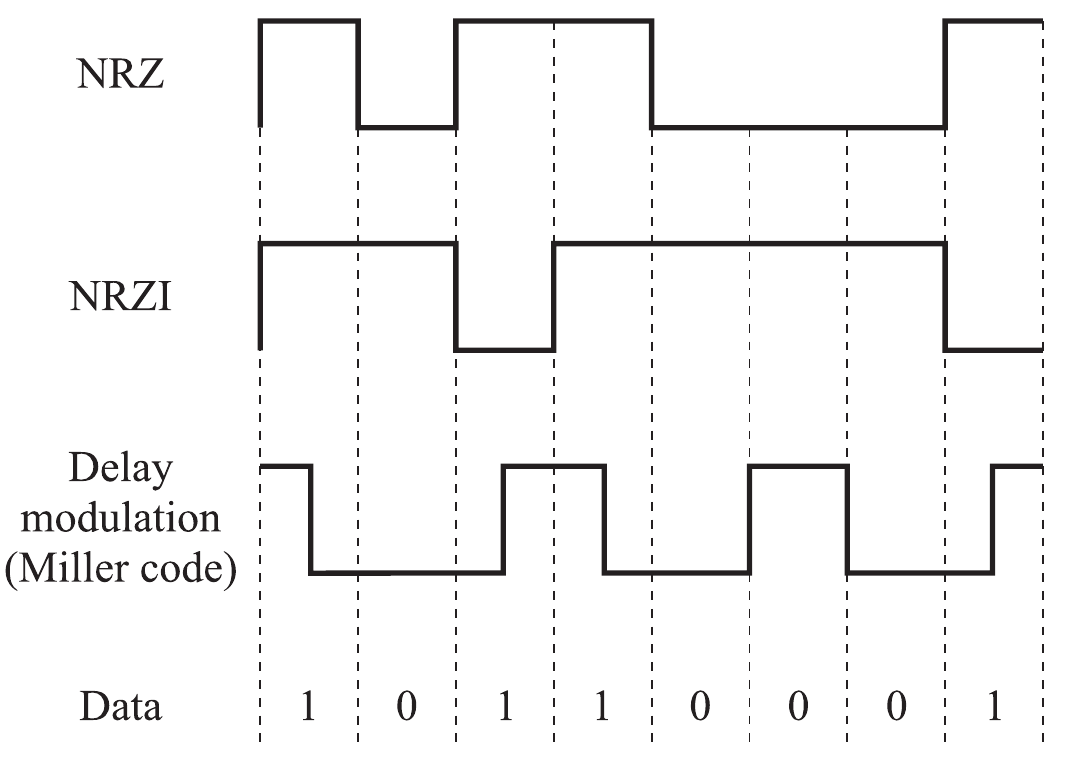
\includegraphics[width=0.4\columnwidth]{figs/pam_35}
		\end{center} 
	    \end{figure}
	\end{itemize}
\end{frame}

\begin{frame}
	\frametitle{Estudo de caso: sinal NRZI}

	\begin{itemize}
	    \item Modelagem como cadeia de Markov de dois estados.
	    \item De forma geral, para o caso binário: $P[a_k=1]=1-P[a_k=0]=p$.
	    \item Matriz de transição de estados e diagrama correspondente:
	    \begin{columns}
		\begin{column}{0.35\textwidth}
		    \begin{equation*}
			\mathbf{P} = \left[ \begin{array}{cc} 1-p & p \\ p & 1-p \end{array} \right]
		    \end{equation*}
		\end{column}
		\begin{column}{0.65\textwidth}
		     \begin{figure}[t]	
		      \begin{center}
			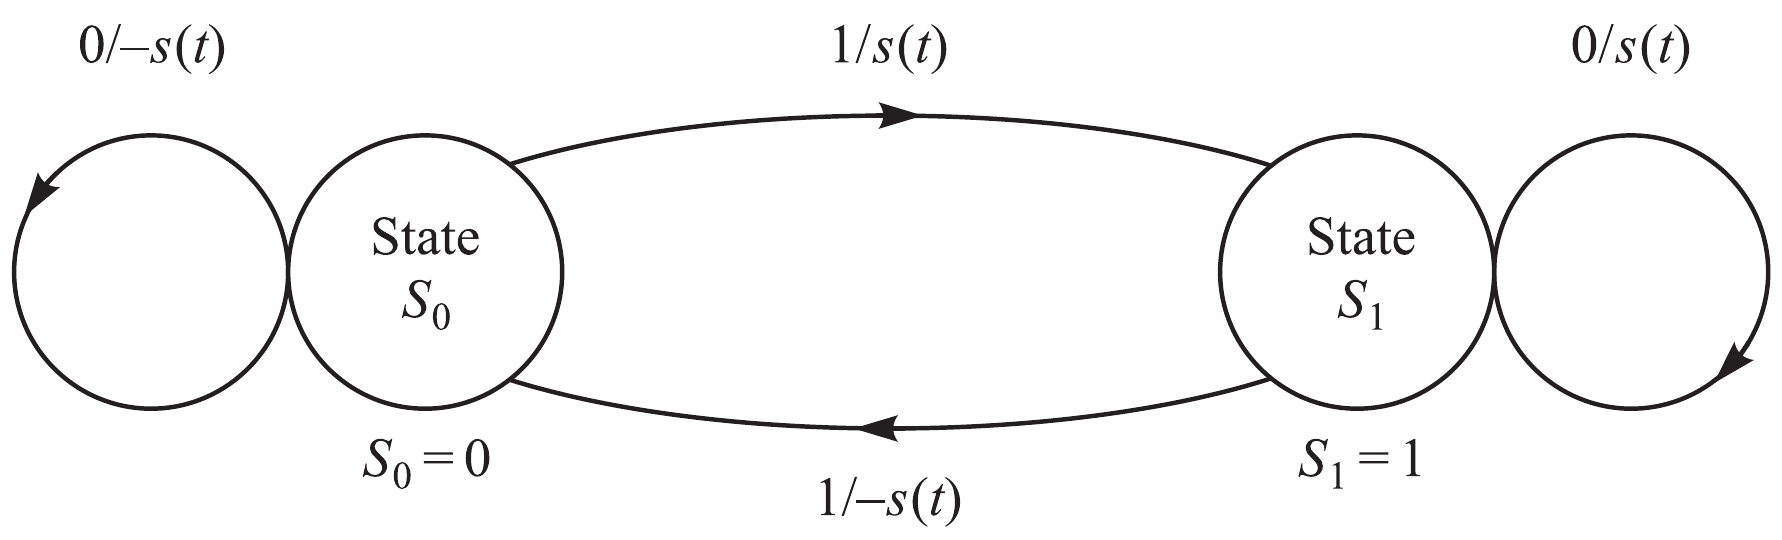
\includegraphics[width=0.85\columnwidth]{figs/pam_36}
		      \end{center}
		    \end{figure}
		\end{column}
	    \end{columns}	 
	    \item Diagrama de treliça (evolução temporal):
	    \begin{figure}[t]	
	      \begin{center}
		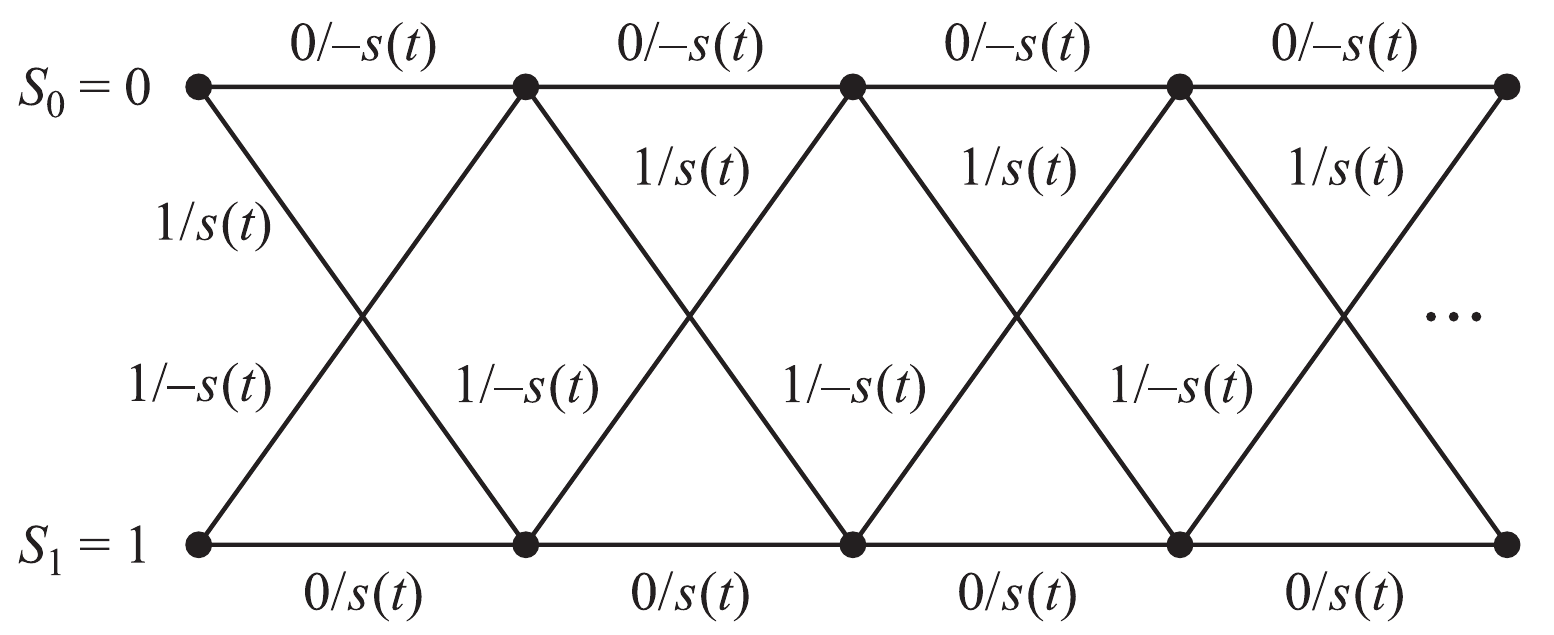
\includegraphics[width=0.5\columnwidth]{figs/pam_37}
	      \end{center}
	    \end{figure}
	\end{itemize}
\end{frame}

\begin{frame}
	\frametitle{Algoritmo de Viterbi}

	\begin{itemize}
	    \item Considere um sinal PAM binário NRZI, com $s_1 = -s_2 = \sqrt{\mathcal{E}_b}$.
	    \item Número total de possíveis sequências $2^L$.
	    \item Algoritmo de Viterbi reduz a complexidade eliminando sequências de forma iterativa: algoritmo de busca em treliça.
	    \item Diagrama em treliça supondo estado inicial $S_0$.	    
	\end{itemize}
	\begin{figure}[t]	
	  \begin{center}
	    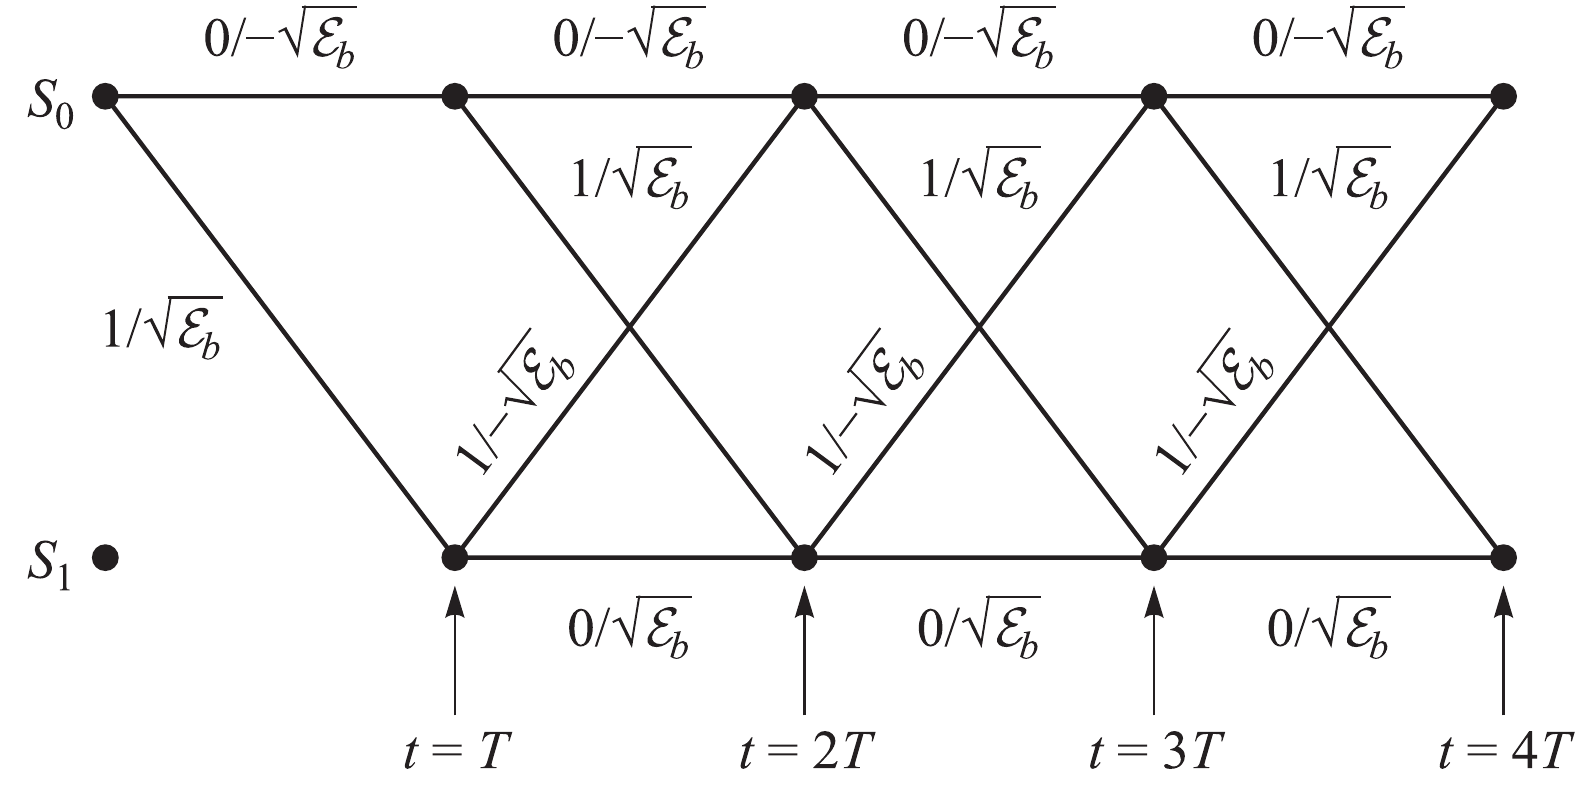
\includegraphics[width=0.5\columnwidth]{figs/pam_38}
	  \end{center}
	\end{figure}
\end{frame}

\begin{frame}
	\frametitle{Algoritmo de Viterbi}

	\vspace{-0.3cm}
	\begin{figure}[t]	
	  \begin{center}
	    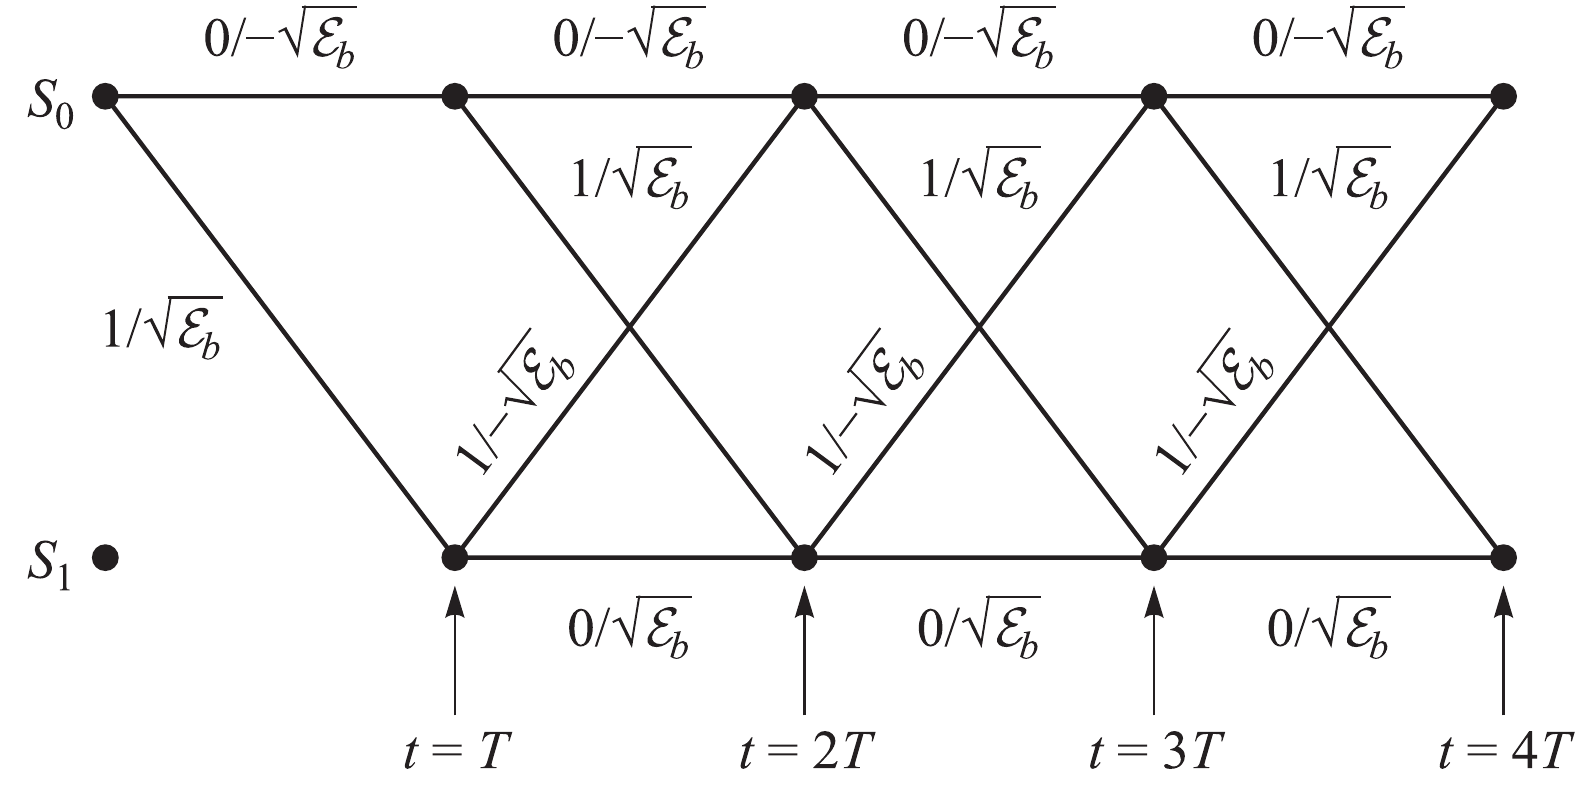
\includegraphics[width=0.5\columnwidth]{figs/pam_38}
	  \end{center}\vspace{-0.5cm}
	\end{figure}
	\begin{itemize}
	    \item Memória de 1 bit, treliça atinge estado permanente após 2 transições.
	    \item Em $t=2T$ há dois caminhos entrando em cada nó.
	    \item Métricas de decisão para o nó $S_0$ baseadas em distância Euclidiana:
	    \begin{align*}
		D_0(0,0) &= (r_1 + \sqrt{\mathcal{E}_b})^2 + (r_2 + \sqrt{\mathcal{E}_b})^2 \\
		D_0(1,1) &= (r_1 - \sqrt{\mathcal{E}_b})^2 + (r_2 + \sqrt{\mathcal{E}_b})^2
	    \end{align*}
	    \item Caminho de menor métrica é escolhido e o outro é descartado.
	\end{itemize}
\end{frame}

\begin{frame}
	\frametitle{Algoritmo de Viterbi}

	\vspace{-0.3cm}
	\begin{figure}[t]	
	  \begin{center}
	    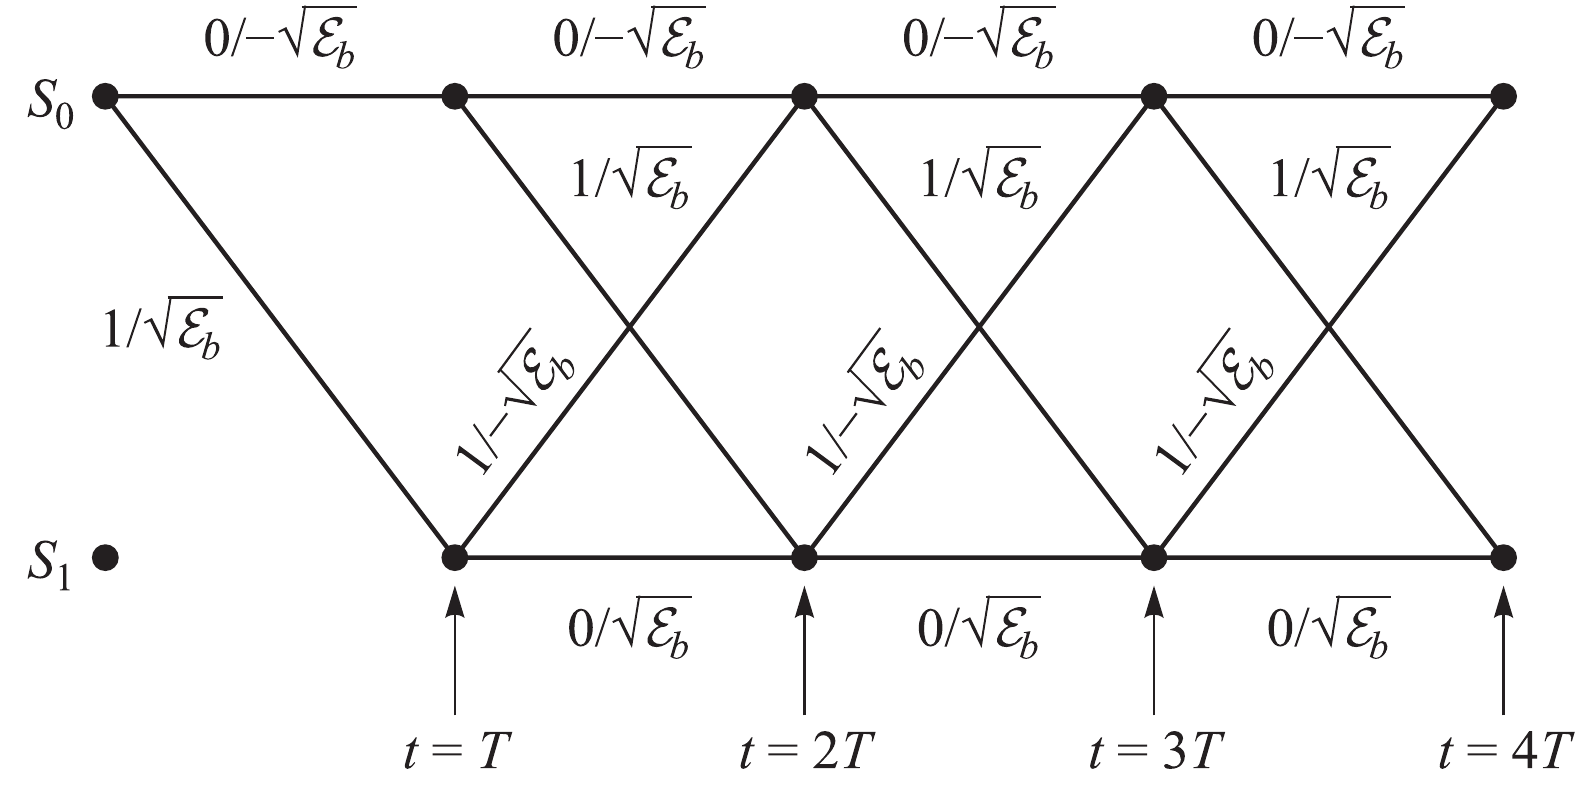
\includegraphics[width=0.5\columnwidth]{figs/pam_38}
	  \end{center}\vspace{-0.5cm}
	\end{figure}
	\begin{itemize}
	    \item Mesmo procedimento para o nó $S_1$ ainda em $t=2T$
	    \begin{align*}
		D_1(0,1) &= (r_1 + \sqrt{\mathcal{E}_b})^2 + (r_2 - \sqrt{\mathcal{E}_b})^2 \\
		D_1(1,0) &= (r_1 - \sqrt{\mathcal{E}_b})^2 + (r_2 - \sqrt{\mathcal{E}_b})^2
	    \end{align*}
	    \item Em $t=2T$ ficamos portanto com um caminho sobrevivente chegando em cada nó.
	\end{itemize}
\end{frame}

\begin{frame}
	\frametitle{Algoritmo de Viterbi}

	\vspace{-0.3cm}
	\begin{figure}[t]	
	  \begin{center}
	    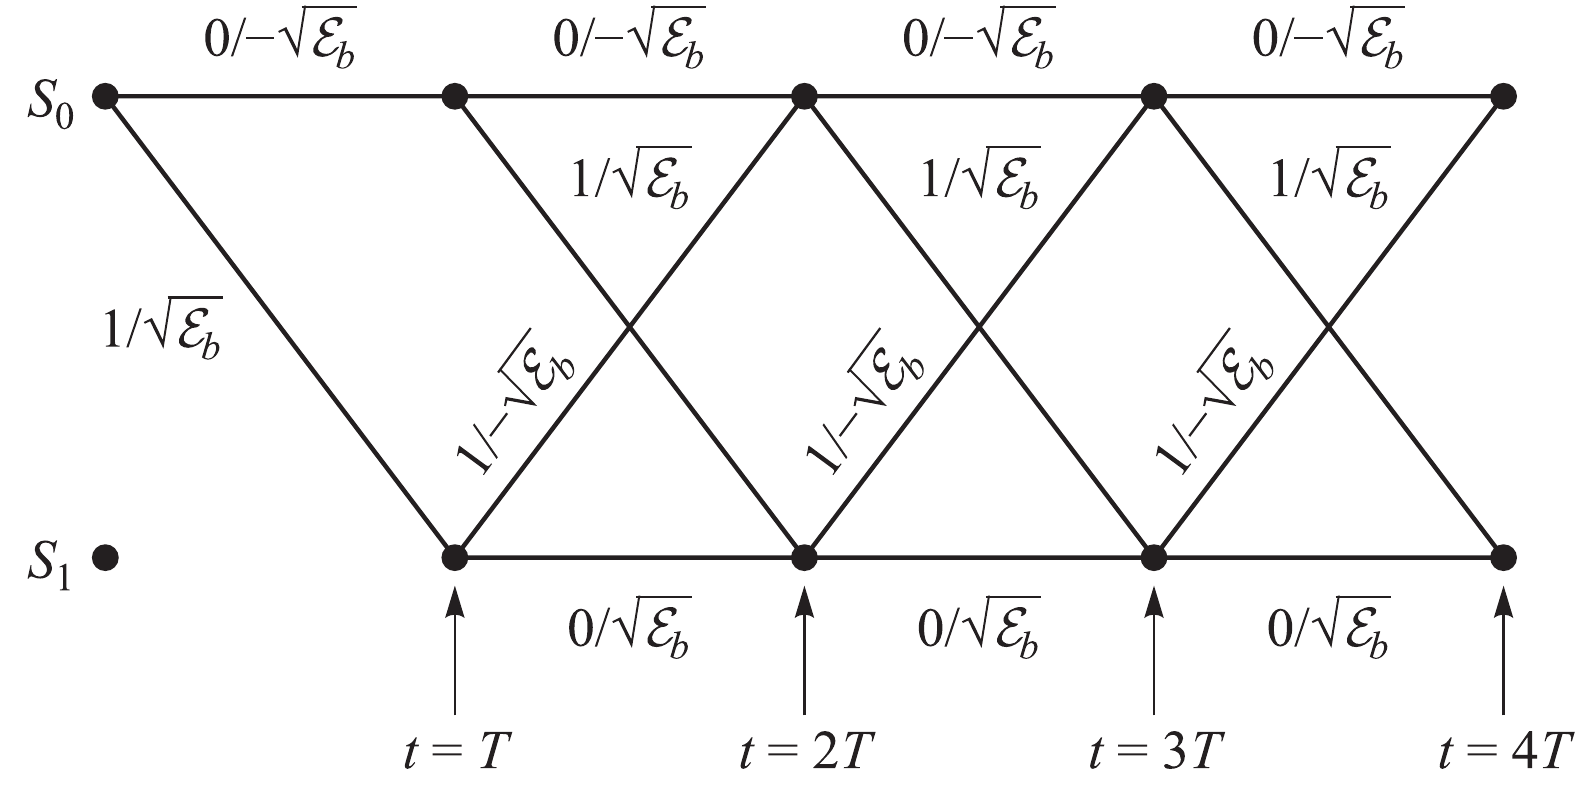
\includegraphics[width=0.5\columnwidth]{figs/pam_38}
	  \end{center}\vspace{-0.5cm}
	\end{figure}
	\begin{itemize}
	    \item Supondo que os caminhos sobreviventes em $t=2T$ sejam $(0,0)$ em $S_0$ e $(0,1)$ em $S_1$.
	    \item As métricas em $t=3T$ são calculadas como:
	    \begin{small}
	    \begin{align*}
		D_0(0,0,0) &= D_0(0,0) + (r_3 + \sqrt{\mathcal{E}_b})^2 \qquad D_1(0,0,1) = D_0(0,0) + (r_3 - \sqrt{\mathcal{E}_b})^2 \\
		D_0(0,1,1) &= D_1(0,1) + (r_3 + \sqrt{\mathcal{E}_b})^2 \qquad D_1(0,1,0) = D_1(0,1) + (r_3 - \sqrt{\mathcal{E}_b})^2
	    \end{align*}
	    \end{small}
	    \item Novamente é escolhido o caminho de menor métrica em cada nó.
	\end{itemize}
\end{frame}

\begin{frame}
	\frametitle{Algoritmo de Viterbi}

	\begin{figure}[t]	
	  \begin{center}
	    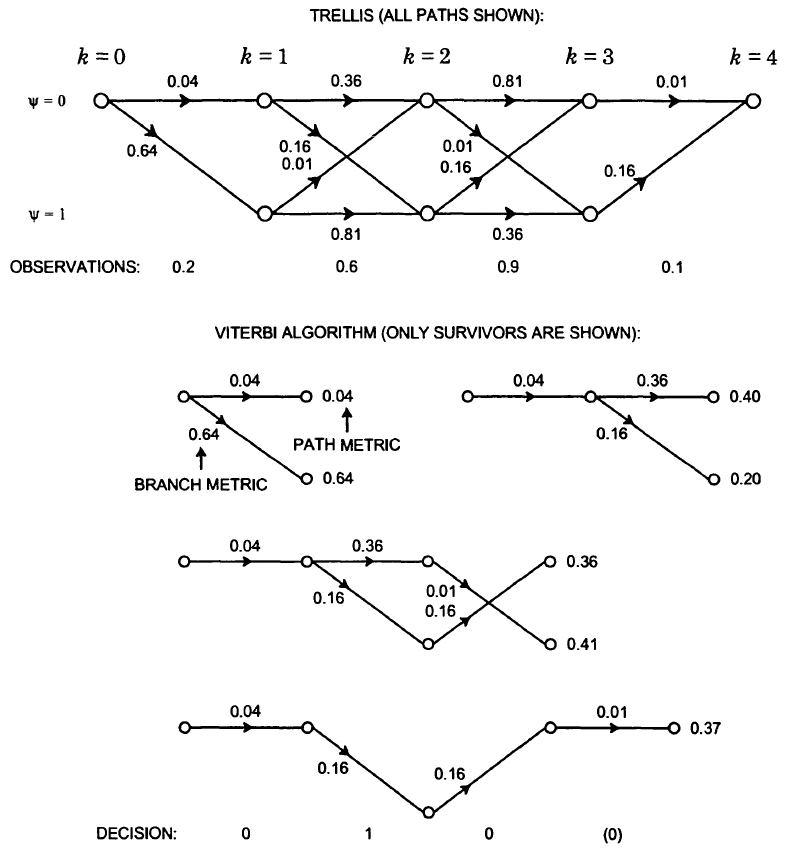
\includegraphics[width=0.58\columnwidth]{figs/pam_40}
	  \end{center}
	\end{figure}
\end{frame}

\begin{frame}
	\frametitle{Algoritmo de Viterbi}

	\begin{itemize}
	    \item O processo continua a cada tempo de símbolo.
	    \item O número de caminhos na treliça é reduzido pela metade a cada estágio.
	    \item Pode ser generalizado para modulação $M$-ária.
	    \item A escolha do tamanho da sequência para realizar a decisão depende da memória (e.g., número de multi-percursos em canal rádio móvel).
	    \item Supondo que a memória tem comprimento $L_m$, uma implementação prática do algoritmo geralmente considera sequências de tamanho $L=5L_m$.
	    \item Desta forma é possível compensar o efeito da memória e evitar um atraso muito grande na entrega dos símbolos no receptor.
	\end{itemize}
\end{frame}

\begin{frame}
	\frametitle{Algoritmo de Viterbi}

	\begin{itemize}
	    \item Exemplo para 4-PSK, canal com memória de tamanho 2.
	\end{itemize}
	\begin{figure}[t]	
	  \begin{center}
	    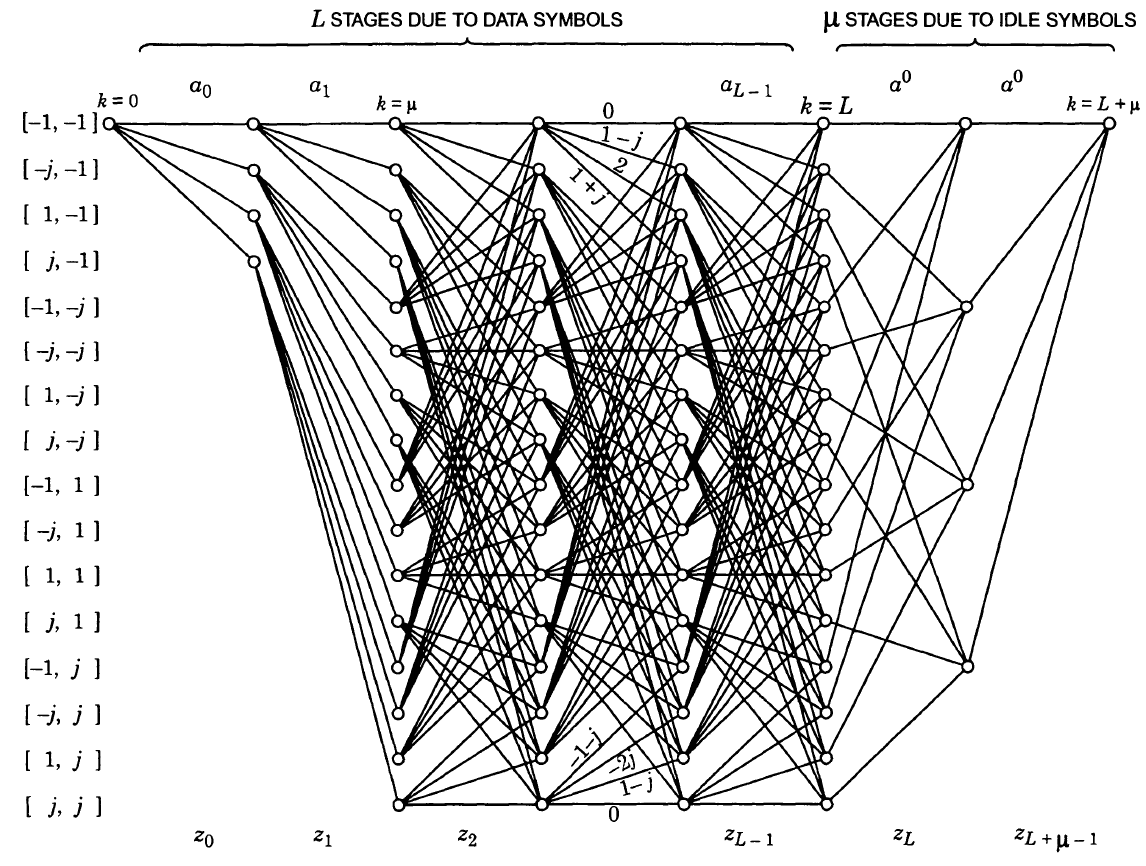
\includegraphics[width=0.76\columnwidth]{figs/pam_39}
	  \end{center}
	\end{figure}
\end{frame}

% \begin{frame}
% 	\frametitle{Minimização da distância para tempo discreto}
% 
% 	\begin{itemize}
% 	    \item Cálculo direto do custo $J$ não é prático: 
% 	    \begin{itemize}
% 	     \item Para uma sequência requer por volta de $L^2$ operações e o número de sequências cresce exponencialmente com $L$.
% 	    \end{itemize}
% 	    \item Conversão do critério de distância mínima de tempo contínuo para tempo discreto:
% 	    \begin{figure}[t]	
% 		\begin{center}
% 		\includegraphics[width=0.75\columnwidth]{figs/pam_34}
% 		\end{center} 
% 	    \end{figure}
% 	    \item Problema equivalente:
% 	    \begin{equation*}
% 		\hat{\mathcal{S}}_k = \arg \max_{\mathcal{S} \in \mathcal{A}^L} \; \sum_{k=0}^{\infty} \left| z_k - \sum_{l=0}^{L-1} a_l m_{k-l} \right|^2
% 	    \end{equation*}
% 	\end{itemize}
% \end{frame}
% 
% \begin{frame}
% 	\frametitle{Minimização da distância para tempo discreto}
% 
% 	\begin{itemize}
% 	    \item Fatorização espectral
% 	    \begin{align*}
% 		&S_h(z) = \gamma^2 M(z) M^*(1/z^*) \\
% 		&\rho_h(k) = \gamma^2 m_k * m_{-k}^* \\
% 		&\text{Função de transferência do equalizador precursor: } \frac{1}{\gamma^2 M^*(1/z^*)} \\
% 		&y_k = \gamma^2 z_k * m_{-k}^* = \gamma^2 \sum_{l=k}^{\infty} z_l m_{l-k}^* \\
% 		
% 	    \end{align*}    
% 	\end{itemize}
% \end{frame}

\section{Análise de Desempenho em canais AWGN}

\begin{frame}
	\frametitle{Probabilidade de erro de símbolo}

	\begin{itemize}
	    \item Análise de desempenho do PAM em banda passante na presença de ruído aditivo Gaussiano branco (AWGN).
	    \item Considere um pulso PAM isolado (ou uma sequência de pulsos que satisfazem o critério de Nyquist).
	    \item Cadeia de transmissão e recepção:
	    \begin{figure}[t]	
	      \begin{center}
		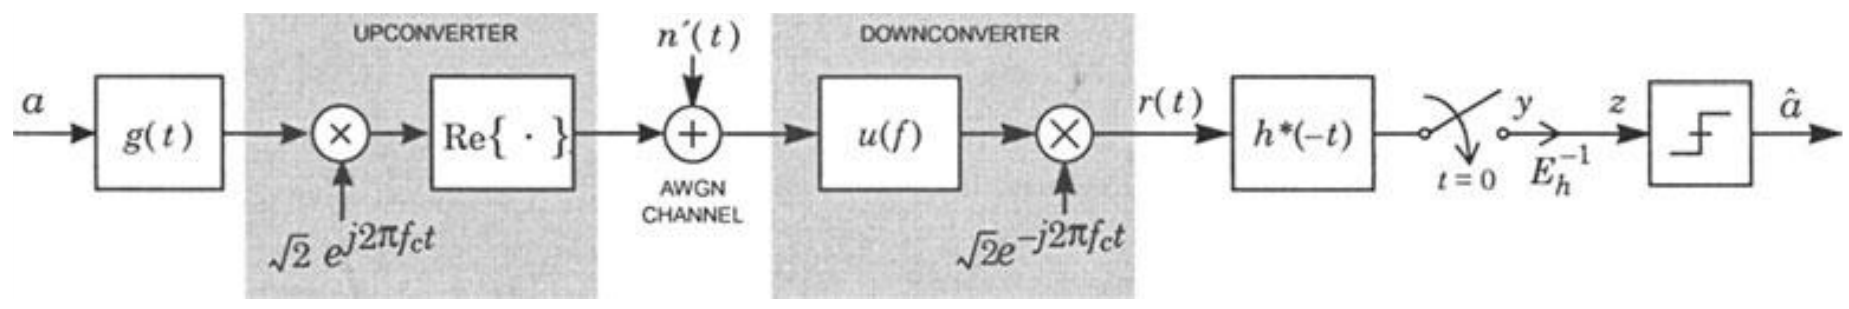
\includegraphics[width=0.85\columnwidth]{figs/pam_41}
	      \end{center}
	    \end{figure}
	    \item Sinal recebido:
	    \begin{equation*}
		  r(t) = ah(t) + n(t)
	    \end{equation*}
	    \item Onde $a\in \mathcal{A}$, $h(t)$ é o pulso recebido e $n(t)$ o ruído recebido.
	\end{itemize}	
\end{frame}

\begin{frame}
	\frametitle{Probabilidade de erro de símbolo}

	\begin{itemize}
	    \item Caracterização estatística do ruído.
	    \item Considere que $n'(t)$ é o ruído antes da translação de frequência: real, Gaussiano, branco e com DEP $N_0/2$.
	    \begin{figure}[t]	
	      \begin{center}
		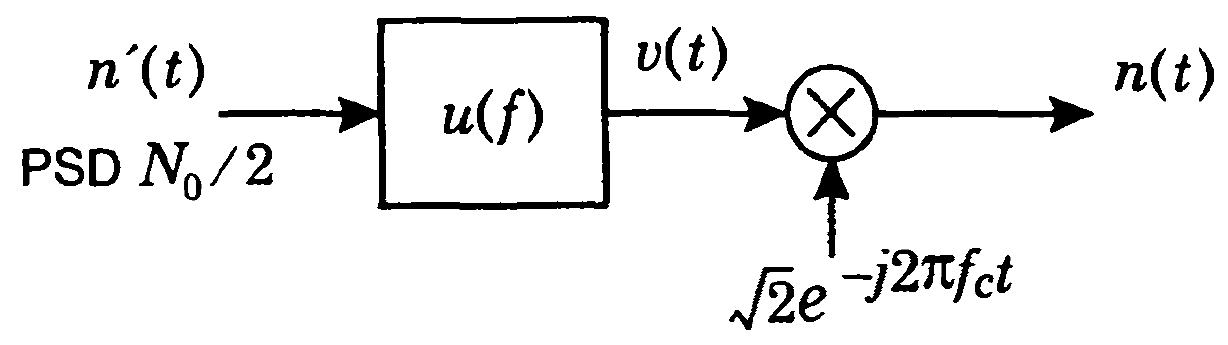
\includegraphics[width=0.45\columnwidth]{figs/pam_42}
	      \end{center}
	    \end{figure}
	    \item Cálculo da DEP do ruído filtrado em $v(t)$ e $n(t)$:
	    \begin{equation*}
		S_v(f) = (N_0/2)u(f) \qquad \text{e} \qquad S_n(f) = N_0u(f+f_c)
	    \end{equation*}
	    \item Considerando um receptor com filtro casado a saída terá DEP igual a $N_0 |H(f)|^2$.
	\end{itemize}	
\end{frame}

\begin{frame}
	\frametitle{Probabilidade de erro de símbolo}

	\begin{itemize}
	    \item Considerando o filtro casado, o sinal recebido normalizado é dado por:
	    \begin{align*}
		   z &= \mathcal{E}_h^{-1}\int_{-\infty}^{\infty} r(t) h^*(t) dt =  \mathcal{E}_h^{-1}\int_{-\infty}^{\infty} (ah(t) + n(t)) h^*(t) dt \\ &= a\mathcal{E}_h^{-1}\underbrace{\int_{-\infty}^{\infty} h(t) h^*(t) dt}_{\mathcal{E}_h} + \underbrace{\mathcal{E}_h^{-1}\int_{-\infty}^{\infty} n(t) h^*(t) dt}_{n} = a + n
	    \end{align*}
	    \item A variável complexa $n$ possui distribuição $\mathcal{CN}(0,N_0/\mathcal{E}_h)$
	    \item Processo similar pode ser aplicado para o PAM em banda base.
	\end{itemize}	
\end{frame}

\begin{frame}
	\frametitle{Probabilidade de erro de símbolo}

	\begin{itemize}
	    \item Relação sinal-ruído:
	    \begin{equation*}
		    \mathrm{SNR} = \frac{\mathrm{E}[|a|^2]}{\mathrm{E}[|n|^2]} = \frac{\mathcal{E}_a}{N_0/\mathcal{E}_h} = \frac{\mathcal{E}_a\mathcal{E}_h}{N_0}
	    \end{equation*}
	    \item Detecção: $z$ é aplicado a um \textit{slicer}, o qual escolher o símbolo $a \in \mathcal{A}$ que minimiza $|z-a|^2$.
	    \item Um \textbf{erro de símbolo} ocorre quando o \textit{slicer} escolhe um símbolo diferente daquele que foi de fato transmitido.
	    \item Vamos determinar a probabilidade de que o receptor de distância mínima cometa um erro de decisão em cenário AWGN.
	\end{itemize}	
\end{frame}

\begin{frame}
	\frametitle{Probabilidade de erro de símbolo}

	\begin{itemize}
	    \item Exemplo de detecção do \textcolor{blue}{BPSK}, para $\mathcal{A}=\{\pm \sqrt{\mathcal{E}_a} \}$
	    \item Supondo que o símbolo negativo foi transmitido, obtemos a PDF de $z$:
	    \begin{figure}[t]	
	      \begin{center}
		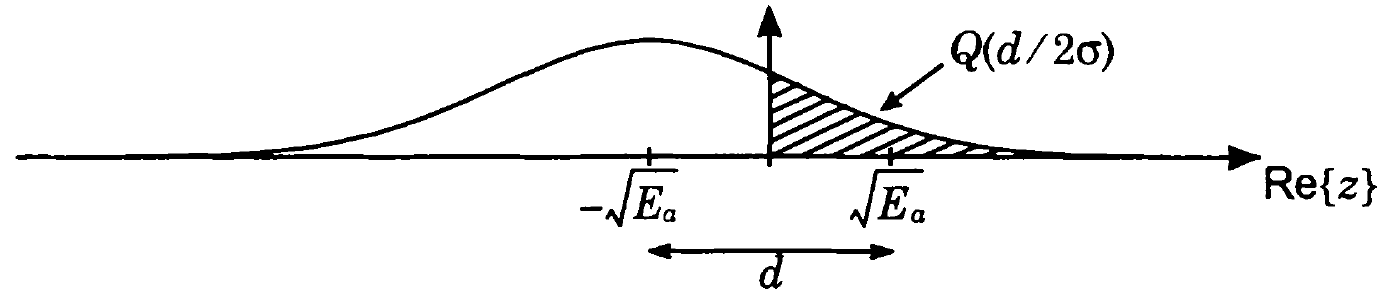
\includegraphics[width=0.6\columnwidth]{figs/pam_43}
	      \end{center}
	    \end{figure}
	    \item Distribuição de $z$: $\mathcal{N}(-\sqrt{\mathcal{E}_a},\sigma^2)$
	    \item Variância do ruído por dimensão: $\sigma^2 = N_0/(2\mathcal{E}_h)$
	    \item Distância entre símbolos: $d=2\sqrt{\mathcal{E}_a}$
	    \item Probabilidade de erro de símbolo:
	    \begin{equation*}
		    \mathrm{Pr[erro]} = Q(d/2\sigma) = Q(\sqrt{2\mathcal{E}/N_0})
	    \end{equation*}
	    \item Neste caso a probabilidade de erro de símbolo é igual à de erro de bit.
	\end{itemize}	
\end{frame}

\begin{frame}
	\frametitle{Probabilidade de erro de símbolo}

	\begin{itemize}
	    \item Exemplo de detecção do \textcolor{blue}{4-PAM}, para $\mathcal{A}=\{\pm c, \pm 3c \}$ e $c=\sqrt{\mathcal{E}_a/5}$
	    \item Supondo que o símbolo $-c$ foi transmitido, obtemos a PDF de $z$:
	    \begin{figure}[t]	
	      \begin{center}
		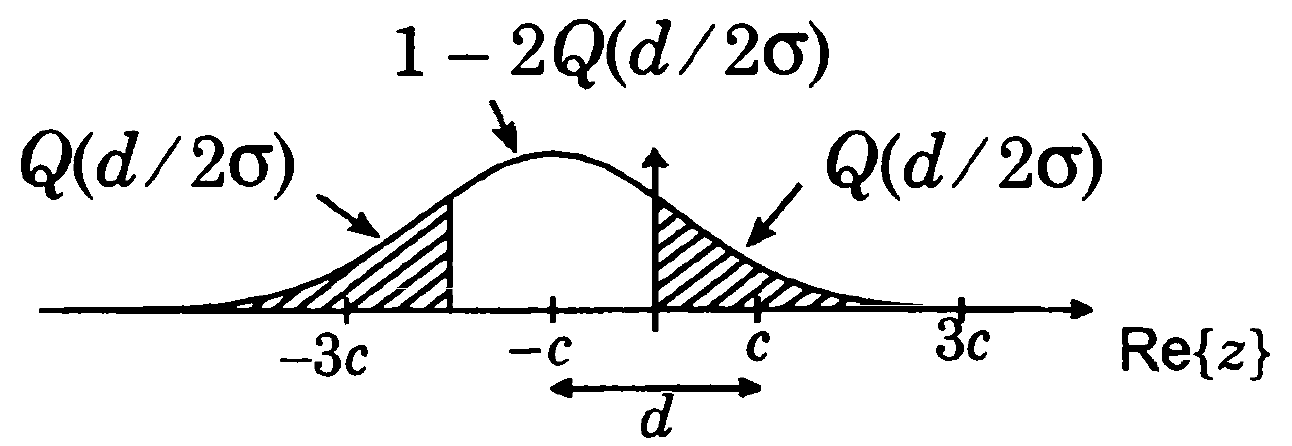
\includegraphics[width=0.43\columnwidth]{figs/pam_44}
	      \end{center}
	    \end{figure}
	    \item Cálculo da probabilidade de erro de símbolo:
	    \begin{footnotesize}
	    \begin{align*}
		    \text{Pr[erro}|a=\pm c] &= 2Q(d/2\sigma) \\
		    \text{Pr[erro}|a=\pm 3c] &= Q(d/2\sigma) \\
		    \mathrm{Pr}\text{[erro]} &= \frac{3}{2}Q(d/2\sigma) = \frac{3}{2}Q\left(\sqrt{\frac{2}{5}\mathcal{E}/N_0}\right)
	    \end{align*}
	    \end{footnotesize}
	    \item De forma geral, para o \textcolor{blue}{$M$-PAM} temos:
	    \begin{footnotesize}
	    \begin{align*}
		    \mathrm{Pr}\text{[erro]} &= \frac{2(M-1)}{M}Q\left(\sqrt{\frac{6}{(M^2-1)}\mathcal{E}/N_0}\right)
	    \end{align*}
	    \end{footnotesize}
	\end{itemize}	
\end{frame}

\begin{frame}
	\frametitle{Probabilidade de erro de símbolo}

	\begin{itemize}
	    \item Exemplo de detecção do \textcolor{blue}{4-QAM}, para $\mathcal{A}=\{\pm c \pm jc \}$ e $c=\sqrt{\mathcal{E}_a/2}$
	    \item Supondo que o símbolo $-c-jc$ foi transmitido:
	    \begin{figure}[t]	
	      \begin{center}
		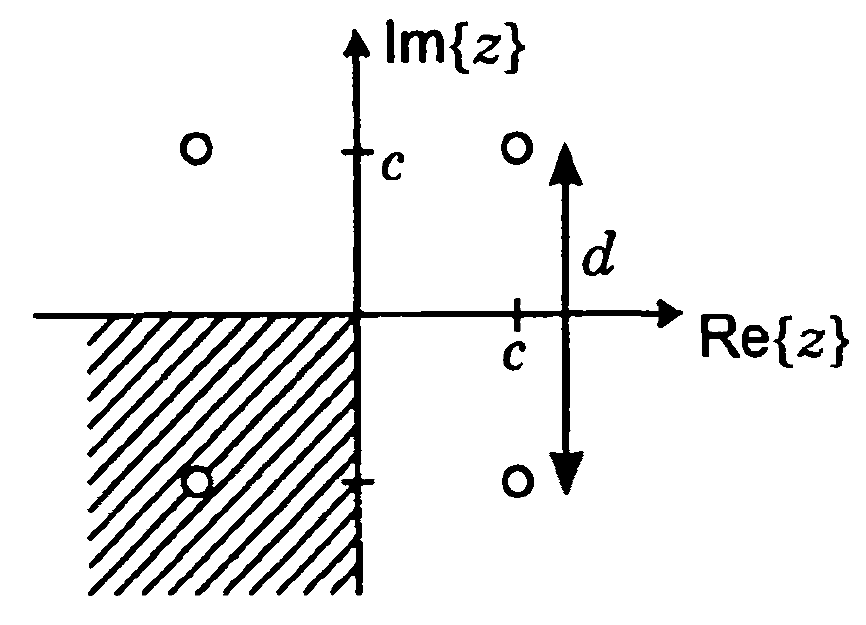
\includegraphics[width=0.3\columnwidth]{figs/pam_45}
	      \end{center}
	    \end{figure}
	    \item Cálculo da probabilidade de erro de símbolo:
	    \begin{footnotesize}
	    \begin{align*}
		    &\text{Pr[acerto}|a=-c-jc] = \mathrm{Pr}[\mathrm{Re}\{z\}<0, \mathrm{Im}\{z\}<0] = (1-Q(d/2\sigma))^2 \\
		    &\text{Pr[erro]} = 1 - \text{Pr[acerto]} = 2Q(d/2\sigma) - Q^2(d/2\sigma) = 2Q(\sqrt{\mathcal{E}/N_0}) - Q^2(\sqrt{\mathcal{E}/N_0}) \\
		    &\text{Aproximação para altos valores de SNR: } \text{Pr[erro]}\approx 2Q(\sqrt{\mathcal{E}/N_0})
	    \end{align*}
	    \end{footnotesize}
	    \item O \textcolor{blue}{4-PSK}, para $\mathcal{A}=\{\pm b, \pm jb \}$ e $b=\sqrt{\mathcal{E}_a}$, corresponde a uma rotação de $45^o$ do 4-QAM, possuindo o mesmo desempenho.
	\end{itemize}	
\end{frame}

\begin{frame}
	\frametitle{Probabilidade de erro de símbolo}

	\begin{columns}
		\begin{column}{0.6\textwidth}
		    \begin{itemize}
			\item Exemplo de detecção do \textcolor{blue}{16-QAM}, para:
			\begin{footnotesize}
			\begin{align*}
			    \mathcal{A} &=\{\pm c \pm jc, \pm c \pm j3c, \pm 3c \pm jc, \pm 3c \pm j3c  \} \\ 
			    c &=\sqrt{\mathcal{E}_a/10}
			\end{align*}		
			\end{footnotesize}
			\item Definição de regiões: \begin{footnotesize}interna, canto, borda.\end{footnotesize}
		    \end{itemize}
		\end{column}
		\begin{column}{0.4\textwidth}
		    \begin{figure}[t]	
		    \begin{center}
			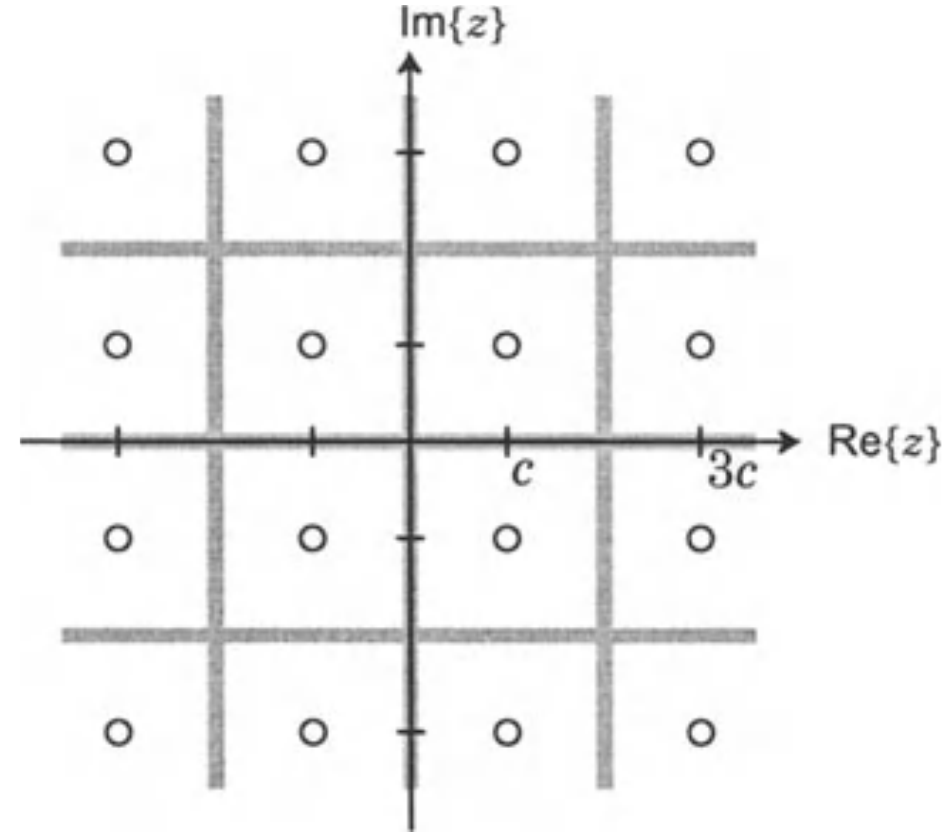
\includegraphics[width=0.8\columnwidth]{figs/pam_46}
		    \end{center}
		    \end{figure}
		\end{column}
	\end{columns}	
	\begin{itemize}
	    \item Cálculo da probabilidade de erro de símbolo:	    
	\end{itemize}	
	\begin{footnotesize}
	\begin{align*}
		&\text{Pr[acerto}|a \text{ interno}] = [1 - 2Q(d/2\sigma)]^2 &\Rightarrow \text{Pr[erro}|a \text{ interno}] \approx 4Q(d/2\sigma) \\
		&\text{Pr[acerto}|a \text{ canto}] = [1 - Q(d/2\sigma)]^2 &\Rightarrow \text{Pr[erro}|a \text{ canto}] \approx 2Q(d/2\sigma) \\
		&\text{Pr[acerto}|a \text{ borda}] = [1 - 2Q(d/2\sigma)][1 - Q(d/2\sigma)] &\Rightarrow \text{Pr[erro}|a \text{ borda}] \approx 3Q(d/2\sigma)
	\end{align*}
	\begin{align*}
		&\text{Pr[erro]} \approx \frac{4}{16}  4Q(d/2\sigma) + \frac{8}{16} 3Q(d/2\sigma) + \frac{4}{16} 2Q(d/2\sigma) = 3Q(d/2\sigma) = 3Q\left(\sqrt{\frac{\mathcal{E}}{5N_0}} \right)
	\end{align*}
	\end{footnotesize}	    
\end{frame}

\begin{frame}
	\frametitle{Probabilidade de erro de símbolo}

	\begin{itemize}
	    \item É possível derivar a expressão \textbf{exata} da probabilidade de erro de símbolo para constelações \textcolor{blue}{$M$-QAM} quadradas, nas quais $M=2^b$ para $b$ par.
	    \item Probabilidade de erro de símbolo do \textcolor{blue}{$\sqrt{M}$-PAM}, com metade da potência alocada em cada dimensão:
	    \begin{small}
	    \begin{equation*}
		\text{Pr[erro]}_{\sqrt{M}} = 2\left(1 - \frac{1}{\sqrt{M}} \right) Q\left(\sqrt{\frac{3\mathcal{E}/N_0}{M-1}} \right)
	    \end{equation*}
	    \item Probabilidade de erro de símbolo do \textcolor{blue}{$M$-QAM}:
	    \end{small}
	    \begin{small}
	    \begin{align*}
		\text{Pr[erro]}_M &= 1 - (1-\text{Pr[erro]}_{\sqrt{M}})^2 \\
		&= 4\left(1 - \frac{1}{\sqrt{M}} \right) Q\left(\sqrt{\frac{3\mathcal{E}/N_0}{M-1}} \right) - 4\left(1 - \frac{1}{\sqrt{M}} \right)^2 Q^2\left(\sqrt{\frac{3\mathcal{E}/N_0}{M-1}} \right) \\
		&\approx 4\left(1 - \frac{1}{\sqrt{M}} \right) Q\left(\sqrt{\frac{3\mathcal{E}/N_0}{M-1}} \right) \quad \text{(para altos valores de SNR)}
	    \end{align*}
	    \end{small}
	\end{itemize}		
\end{frame}

\begin{frame}
	\frametitle{Probabilidade de erro de símbolo}

	\begin{itemize}
	    \item Exemplo de detecção do \textcolor{blue}{$M$-PSK}, para $\mathcal{A}=\{c, ce^{j2\pi/M}, ce^{j4\pi/M}, \ldots, ce^{j2\pi(M-1)/M} \}$ e $c=\sqrt{\mathcal{E}_a}$
	\end{itemize}
	\begin{columns}
		\begin{column}{0.55\textwidth}
		    \begin{itemize}
			\item Região de decisão do símbolo $c$ entre $-\pi/M$ e $\pi/M$.
			\item Expressão fechada não pode ser encontrada.
			\item Cálculo da probabilidade de erro de símbolo:			
			\begin{align*}
			    &P_1 = \text{Pr}[\mathrm{Im}\{n'\} > d/2] = Q(d/2\sigma) \\
			    &n' = ne^{-j\pi/M}			    
			\end{align*}
		    \end{itemize}		    
		\end{column}
		\begin{column}{0.45\textwidth}
		    \begin{figure}[t]	
			\begin{center}\vspace{-0.5cm}
			    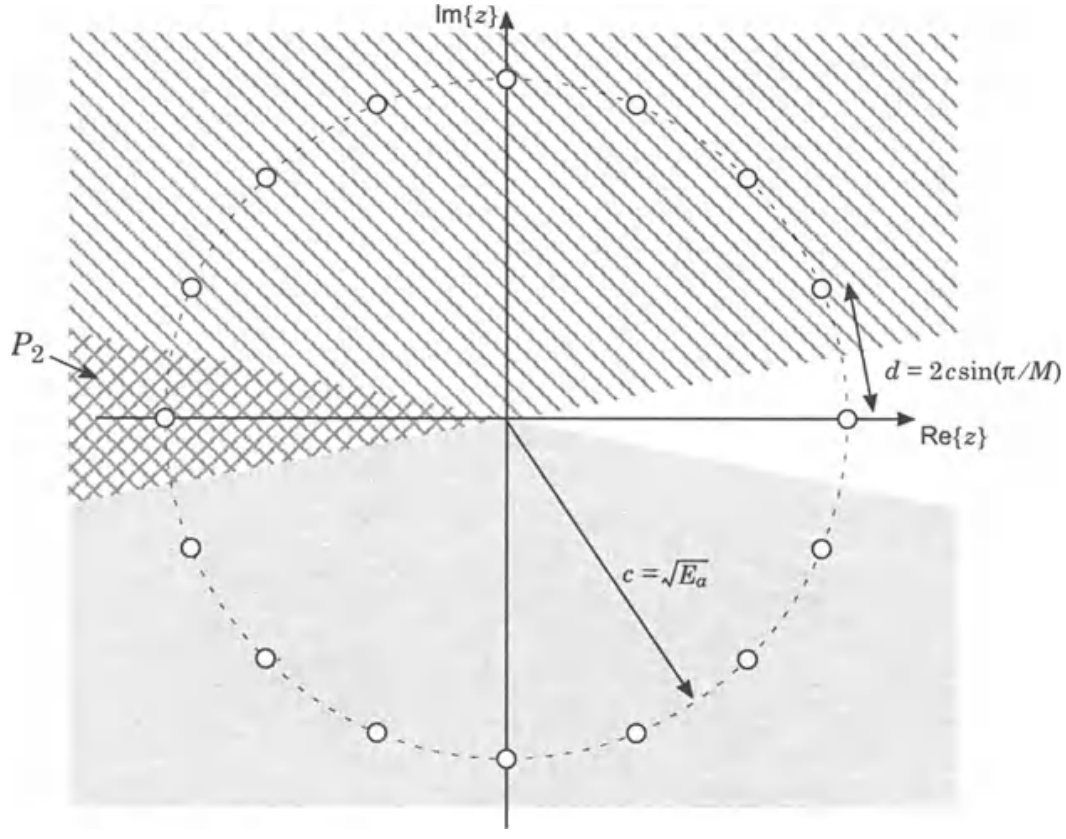
\includegraphics[width=\columnwidth]{figs/pam_47}
			\end{center}
			\end{figure}
		\end{column}
	\end{columns}	    	
	\begin{equation*}\hspace{-1.5cm}
	    \text{Pr[erro]} = 2P_1 - P_2 \approx 2Q(d/2\sigma) \approx2Q\left( \sqrt{2\mathcal{E}/N_0} \sin\frac{\pi}{M} \right)
	\end{equation*}	
\end{frame}


\begin{frame}
	\frametitle{Requisitos de banda e SNR do PAM em banda passante}

	\vspace{-0.3cm}
	\begin{itemize}
	    \item Probabilidade de erro de símbolo foi calculada como função da SNR = $\mathcal{E}/N_0$ para diferentes esquemas de modulação.
	    \item Para permitir a comparação entre esquemas de diferente ordens, é necessário normalizar a energia por bit:
	    \begin{equation*}
		\mathcal{E}_b = \mathcal{E}/\log_2 |\mathcal{A}| = \mathcal{E}/b
	    \end{equation*}
	    \item Razão entre a energia por bit e o ruído: $\mathcal{E}_b / N_0$
	    \item Mapeamento \textit{Gray} reduz a diferença entre símbolos adjacentes.
	\end{itemize}	
	\begin{columns}
		\begin{column}{0.5\textwidth}
		    \begin{itemize}			
			\item Aproximação:
			\begin{small}
			\begin{equation*}
			    \text{Pr[erro de bit]} \approx \frac{1}{b}\text{Pr[erro de símbolo]}
			\end{equation*}
			\end{small}
		    \end{itemize}		    
		\end{column}
		\begin{column}{0.5\textwidth}
		    \begin{figure}[t]	
			\begin{center}\vspace{-0.5cm}
			    \includegraphics[width=\columnwidth]{figs/pam_48}
			\end{center}
		    \end{figure}
		\end{column}
	\end{columns}	
\end{frame}

\begin{frame}
	\frametitle{Requisitos de banda e SNR do PAM em banda passante}

	\begin{itemize}
	    \item Expressões de probabilidade de erro de bit:
	    \begin{alignat*}{2}
		&P_b^{\text{BPSK}} &&= Q(\sqrt{2\mathcal{E}_b/N_0}) \\
		&P_b^{M-\text{QAM}} &&\approx \frac{4}{b} (1-2^{-b/2}) Q\left(\sqrt{\frac{3b\mathcal{E}_b/N_0}{2^b-1}} \right) \\
		&P_b^{M-\text{PSK}} &&\approx \frac{2}{b} Q\left(\sqrt{2b\mathcal{E}_b/N_0} \sin\frac{\pi}{M} \right)
	    \end{alignat*}

	\end{itemize}	
\end{frame}

\begin{frame}[t,fragile]
	\frametitle{Probabilidade de erro de símbolo}

	\begin{itemize}
	    \item Desempenho dos esquemas de modulação (QAM):
	\end{itemize}
	\begin{figure}\vspace{-0.4cm}
  \centering
    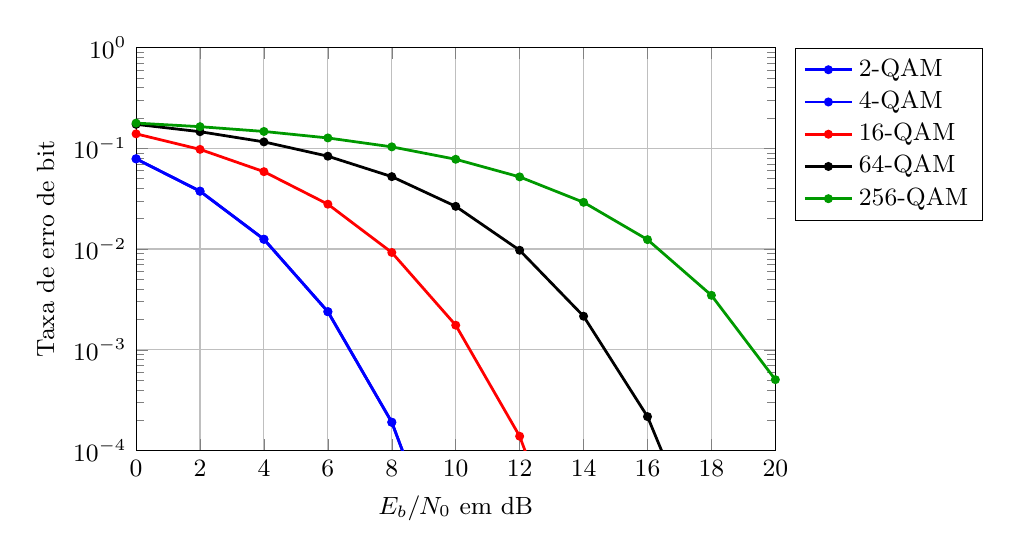
\begin{tikzpicture}
     \begin{axis}[
	    xlabel=$E_b/N_0$ em dB,
	    ylabel=Taxa de erro de bit,
	    ymode=log,
	    yminorticks=true,
 	    grid=major,
	    xmin=0, xmax=20, ymin=1e-4, ymax=1e0,
%   	    ytick={1-6,1e-5,...,1},
	    legend pos=outer north east,
	    legend cell align=left, font=\small,
	    height=6.7cm, width=0.8\columnwidth]
    \addplot[color=blue,mark=*, mark size=1.1pt, line width=1pt] table {
	     0.00000       7.8650e-02
	     2.00000       3.7506e-02
	     4.00000       1.2501e-02
	     6.00000       2.3883e-03
	     8.00000       1.9091e-04
	    10.00000       3.8721e-06
	    12.00000       9.0060e-09
	    14.00000       6.8102e-13
	    16.00000       2.2674e-19
	    18.00000       1.3960e-29
	    20.00000       1.0442e-45
    };
    \addplot[color=blue,mark=*, mark size=1.1pt, line width=1pt] table {
	     0.00000       7.8650e-02
	     2.00000       3.7506e-02
	     4.00000       1.2501e-02
	     6.00000       2.3883e-03
	     8.00000       1.9091e-04
	    10.00000       3.8721e-06
	    12.00000       9.0060e-09
	    14.00000       6.8102e-13
	    16.00000       2.2674e-19
	    18.00000       1.3960e-29
	    20.00000       1.0442e-45
    };
    \addplot[color=red,mark=*, mark size=1.1pt, line width=1pt] table {
	     0.00000       1.3916e-01
	     2.00000       9.7559e-02
	     4.00000       5.8618e-02
	     6.00000       2.7871e-02
 	     8.00000       9.2472e-03
	    10.00000       1.7542e-03
	    12.00000       1.3866e-04
	    14.00000       2.7632e-06
	    16.00000       6.2502e-09
	    18.00000       4.5223e-13
	    20.00000       1.4040e-19
    };
    \addplot[color=black,mark=*, mark size=1.1pt, line width=1pt] table {
	     0.00000       1.7295e-01
	     2.00000       1.4612e-01
	     4.00000       1.1576e-01
 	     6.00000       8.3473e-02
 	     8.00000       5.2320e-02
	    10.00000       2.6533e-02
	    12.00000       9.7240e-03
	    14.00000       2.1540e-03
	    16.00000       2.1717e-04
	    18.00000       6.3511e-06
	    20.00000       2.6339e-08
    };
    \addplot[color=green!60!black,mark=*, mark size=1.1pt, line width=1pt] table {
	     0.00000          1.7789e-01
	     2.00000          1.6391e-01
	     4.00000          1.4691e-01
 	     6.00000          1.2667e-01
 	     8.00000          1.0334e-01
	    10.00000          7.7807e-02
	    12.00000          5.2022e-02
	    14.00000          2.9098e-02
	    16.00000          1.2400e-02
	    18.00000          3.4721e-03
	    20.00000          5.0531e-04
    };    
    \legend{2-QAM, 4-QAM, 16-QAM, 64-QAM, 256-QAM};
     \end{axis}
     \end{tikzpicture}
     \end{figure}
\end{frame}

\begin{frame}[t,fragile]
	\frametitle{Probabilidade de erro de símbolo}

	\begin{itemize}
	    \item Desempenho dos esquemas de modulação (PSK):
	\end{itemize}
	\begin{figure}\vspace{-0.4cm}
  \centering
    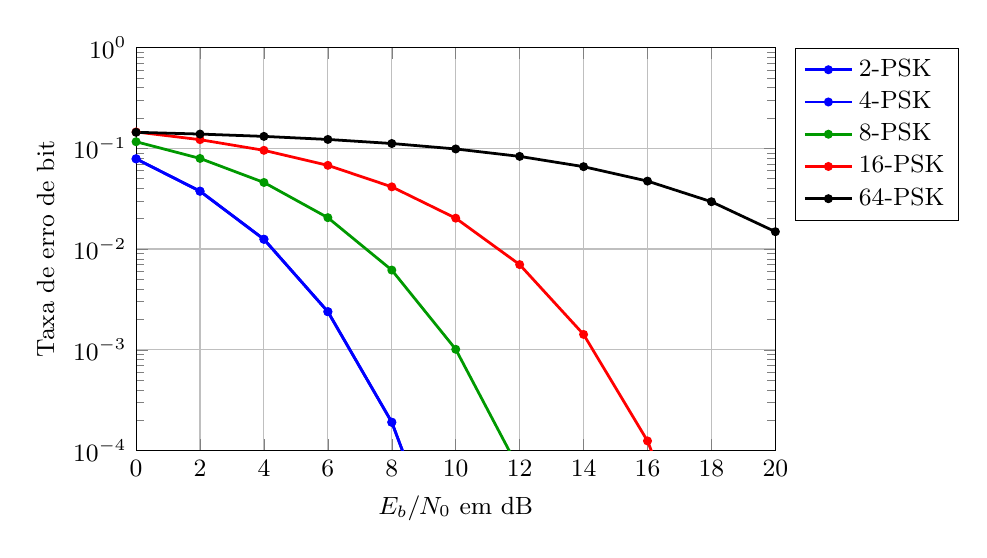
\begin{tikzpicture}
     \begin{axis}[
	    xlabel=$E_b/N_0$ em dB,
	    ylabel=Taxa de erro de bit,
	    ymode=log,
	    yminorticks=true,
 	    grid=major,
	    xmin=0, xmax=20, ymin=1e-4, ymax=1e0,
%   	    ytick={1-6,1e-5,...,1},
	    legend pos=outer north east,
	    legend cell align=left, font=\small,
	    height=6.7cm, width=0.8\columnwidth]
    \addplot[color=blue,mark=*, mark size=1.1pt, line width=1pt] table {
	     0.00000       7.8650e-02
	     2.00000       3.7506e-02
	     4.00000       1.2501e-02
	     6.00000       2.3883e-03
	     8.00000       1.9091e-04
	    10.00000       3.8721e-06
	    12.00000       9.0060e-09
	    14.00000       6.8102e-13
	    16.00000       2.2674e-19
	    18.00000       1.3960e-29
	    20.00000       1.0442e-45
    };
    \addplot[color=blue,mark=*, mark size=1.1pt, line width=1pt] table {
	     0.00000       7.8650e-02
	     2.00000       3.7506e-02
	     4.00000       1.2501e-02
	     6.00000       2.3883e-03
	     8.00000       1.9091e-04
	    10.00000       3.8721e-06
	    12.00000       9.0060e-09
	    14.00000       6.8102e-13
	    16.00000       2.2674e-19
	    18.00000       1.3960e-29
	    20.00000       1.0442e-45
    };
    \addplot[color=green!60!black,mark=*, mark size=1.1pt, line width=1pt] table {
	     0.00000          1.1619e-01      
	     2.00000          7.9321e-02      
	     4.00000          4.5791e-02      
 	     6.00000          2.0480e-02      
 	     8.00000          6.1811e-03      
	    10.00000          1.0114e-03      
	    12.00000          6.3379e-05      
	    14.00000          8.7563e-07      
	    16.00000          1.1099e-09      
	    18.00000          3.2103e-14      
	    20.00000          2.3324e-21      
    }; 
    \addplot[color=red,mark=*, mark size=1.1pt, line width=1pt] table {
	     0.00000          1.4527e-01
	     2.00000          1.2181e-01
	     4.00000          9.5456e-02
	     6.00000          6.7726e-02
 	     8.00000          4.1432e-02
	    10.00000          2.0249e-02
	    12.00000          7.0096e-03
	    14.00000          1.4207e-03
	    16.00000          1.2460e-04
	    18.00000          2.9251e-06
	    20.00000          8.5726e-09
    };
    \addplot[color=black,mark=*, mark size=1.1pt, line width=1pt] table {
	     0.00000          0.144172
	     2.00000          0.138426
	     4.00000          0.131271
 	     6.00000          0.122417
 	     8.00000          0.111568
	    10.00000          0.098486
	    12.00000          0.083101
	    14.00000          0.065712
	    16.00000          0.047251
	    18.00000          0.029494
	    20.00000          0.014863
    };
    \legend{2-PSK, 4-PSK, 8-PSK, 16-PSK, 64-PSK};
     \end{axis}
     \end{tikzpicture}
     \end{figure}
\end{frame}

\begin{frame}
	\frametitle{Requisitos de banda e SNR do PAM em banda passante}

	\begin{itemize}
	    \item A SNR por bit necessária para alcançar um determinado valor de probabilidade de erro de bit pode ser encontrada ao rearranjar as equações anteriores:
	    \begin{align*}
		&(\text{QAM}): \mathcal{E}_b/N_0 = \underbrace{\frac{1}{3}\left(Q^{-1}\left( \frac{bP_b}{4(1-2^{-b/2})} \right) \right)^2}_{\Gamma \text{ (SNR gap)}} \underbrace{\left(\frac{2^b-1}{b}\right)}_{\text{Lim. de Shannon}}  \\ \\
		&(\text{PSK}): \mathcal{E}_b/N_0 = \frac{(Q^{-1}(bP_b/2))^2}{2b\sin^2\frac{\pi}{M}}
	    \end{align*}
	    \item Essas expressões quantificam os requisitos de potência, mas não de banda.
	\end{itemize}	
\end{frame}

\begin{frame}
	\frametitle{Requisitos de banda e SNR do PAM em banda passante}

	\begin{itemize}
	    \item Para o PAM em banda passante, considerando zero de banda de excesso, o requisito de banda é igual à taxa de símbolo. 
	    \item Requisito de banda normalizada: $1/b$
	    \item Comparação entre os esquemas de modulação ($P_b=10^{-6}$):
	    \begin{figure}[t]	
		\begin{center}
		    \includegraphics[width=0.95\columnwidth]{figs/pam_49}
		\end{center}
	    \end{figure}
	\end{itemize}	
\end{frame}